% Created 2024-11-18 Mon 21:08
% Intended LaTeX compiler: pdflatex
\documentclass[11pt]{article}
\usepackage[utf8]{inputenc}
\usepackage[T1]{fontenc}
\usepackage{graphicx}
\usepackage{longtable}
\usepackage{wrapfig}
\usepackage{rotating}
\usepackage[normalem]{ulem}
\usepackage{amsmath}
\usepackage{amssymb}
\usepackage{capt-of}
\usepackage{hyperref}
\usepackage{minted}
\setlength{\parindent}{0em}
\author{Hankertrix}
\date{\today}
\title{Essay on the film "Minority Report"}
\hypersetup{
 pdfauthor={Hankertrix},
 pdftitle={Essay on the film "Minority Report"},
 pdfkeywords={},
 pdfsubject={},
 pdfcreator={Emacs 29.4 (Org mode 9.6.15)}, 
 pdflang={English}}
\makeatletter
\newcommand{\citeprocitem}[2]{\hyper@linkstart{cite}{citeproc_bib_item_#1}#2\hyper@linkend}
\makeatother

\usepackage[notquote]{hanging}
\begin{document}

\maketitle
\setcounter{tocdepth}{2}
\tableofcontents \clearpage
\section{Introduction}
\label{sec:org3b48c5c}
"Minority Report" is a film set in 2054, in the
Washington metropolitan area, and follows John Anderton,
who is the chief of the Precrime department.
The Precrime Department is a specialised police department
that apprehends criminals using foreknowledge provided by
3 psychics, called "Precogs" or "Precognitives".
They are Arthur, Dashiell and Agatha Lively,
with Agatha being the strongest of the three.  \\

In my opinion, the film's setting can be considered
a dystopia, especially for someone like me who is a massive
privacy advocate and holds the individual's freedom in high regard.
There are a lot of problems with how technology is being used in
the film, and it is very concerning that we are seeing some of
it play out in the real world as well.  \\

Let's get into the issues brought up in "Minority Report".

\section{Right to counsel}
\label{sec:orgd4ea62b}
Let's start with one of the first things depicted in the film.
In the opening scene of the film, the judges are invited by
John Anderton to witness the investigation as it progresses
so that the judges can convict and sentence the would-be murderer
immediately once he has been caught.  \\

\begin{figure}[htbp]
\centering
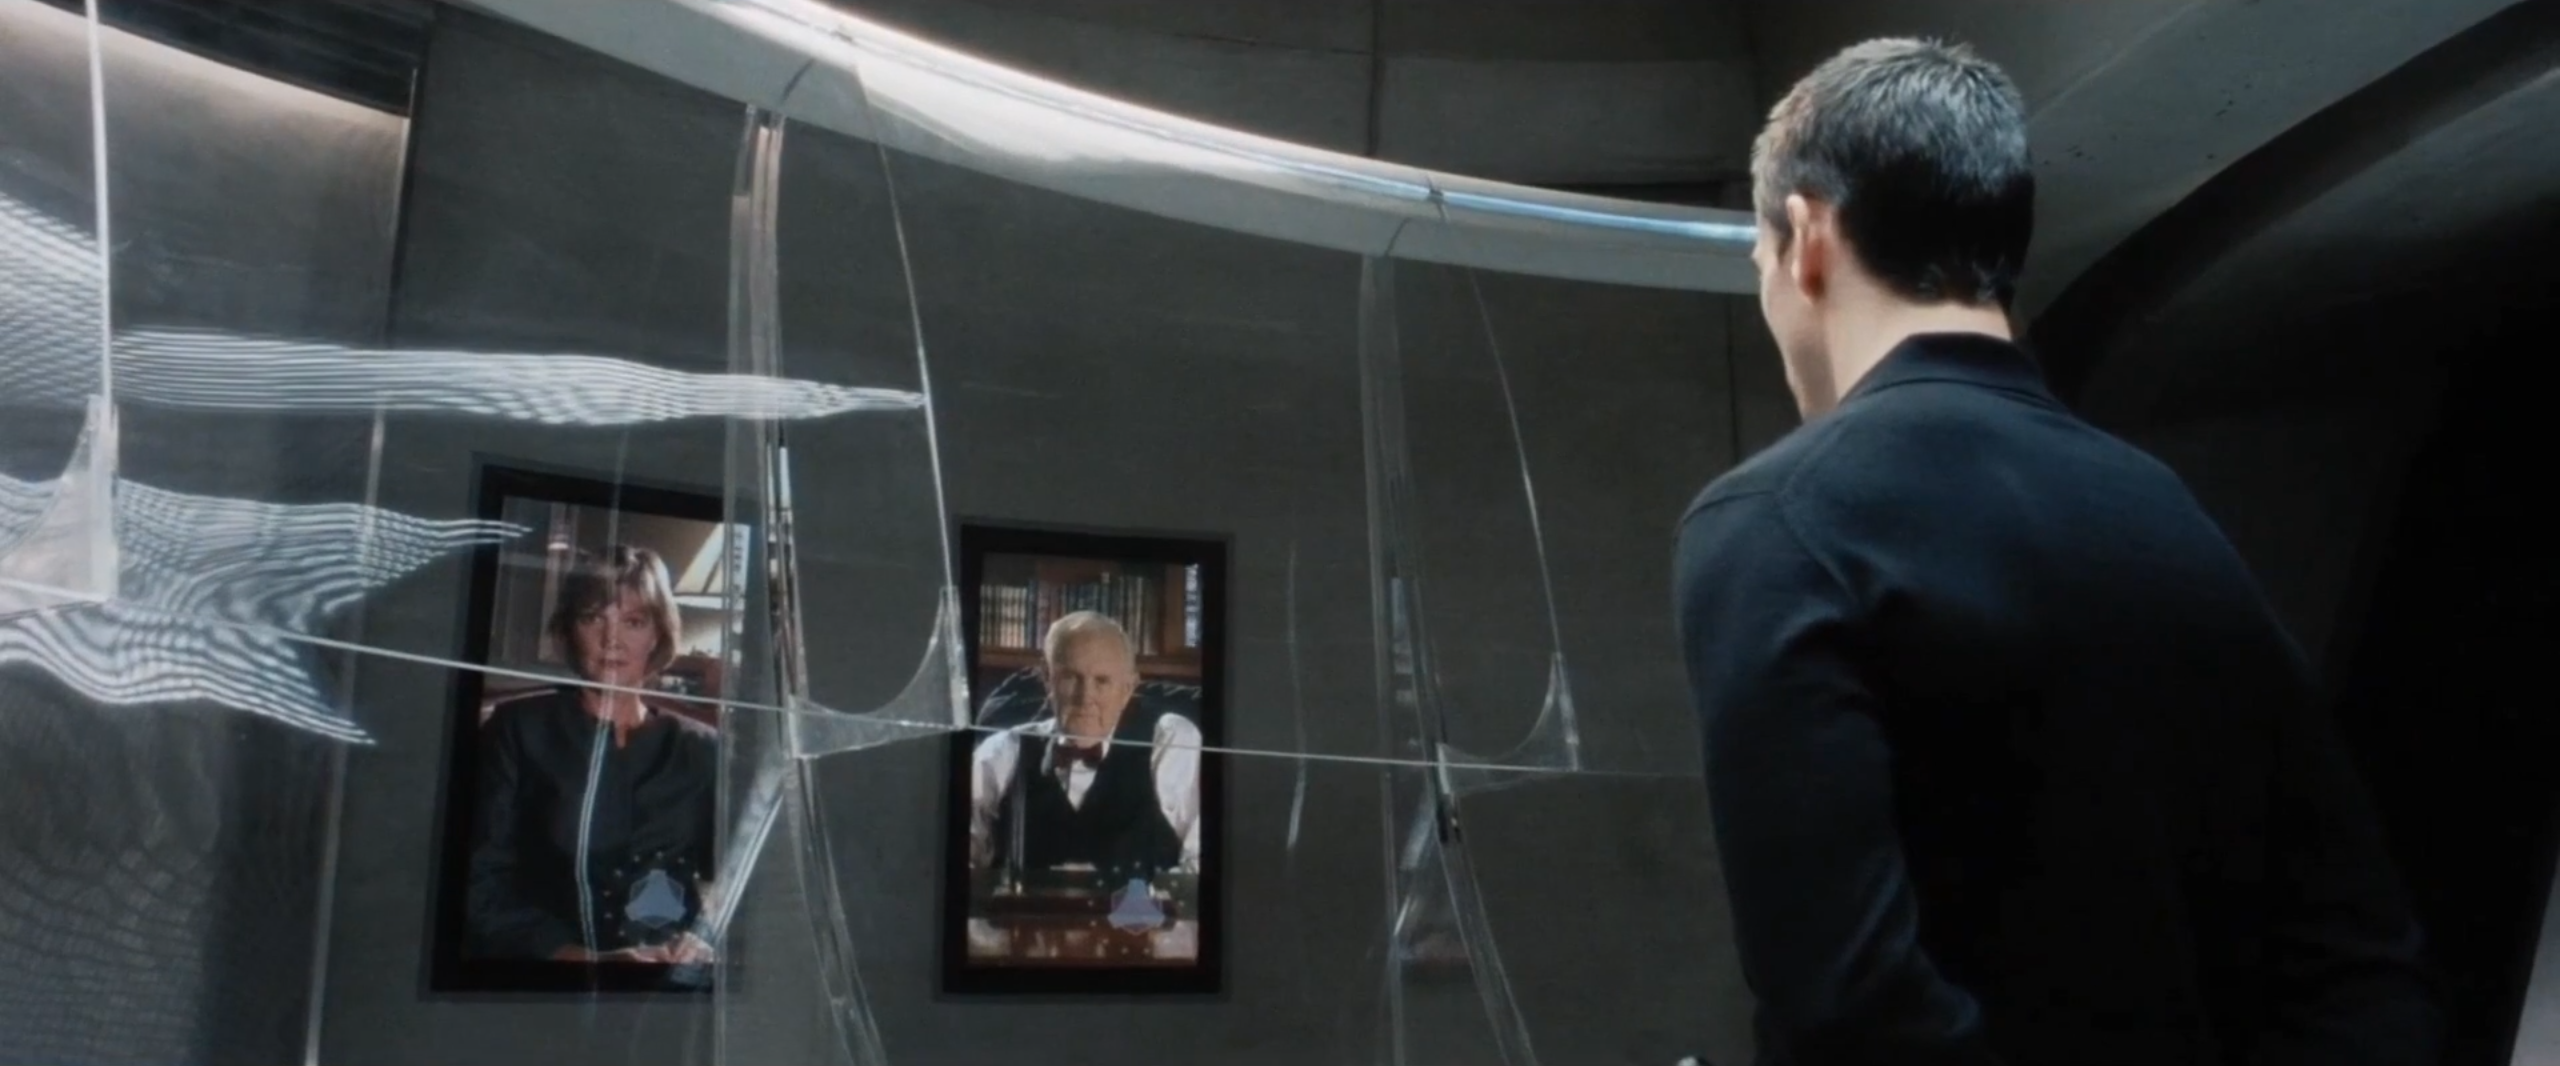
\includegraphics[width=.9\linewidth]{./images/judges-witnessing-and-previewing-the-precognition.png}
\caption{The judges witnessing and previewing the precognition.}
\end{figure}

 \newpage

This means there is no lengthy trial process that the
would-be murderer would have to go through to defend himself
in the court of law, as we see John Anderton immediately putting
the "halo" on the would-be murderer Howard Marks and sending
him straight to the panopticon prison for murder.  \\

This process is due to the absolute belief and trust that Precrime
is infallible and can never be wrong. In such a situation, there
is no need for a would-be murderer to defend himself, since he
definitely would have murdered the person if he had not been stopped,
as the precognition is always 100\% accurate. There is no such thing
as doubt, reasonable or unreasonable since everything is definite,
so there is no need for a trial, and hence, there is no need for a right to counsel.
A trial is only needed for a fallible justice system that has doubt,
so prosecutors will need to prove that the murderer has actually murdered
the person he is accused of murder beyond reasonable doubt.
On the other hand, the murderer will try to prove that he did not murder
the person beyond reasonable doubt, or create sufficient amounts of
reasonable doubt so that the prosecutors cannot prove that he murdered
the person beyond reasonable doubt,
acquitting himself of the murder.  \\

While the absence of the right to counsel seems like a human rights
violation, the trust and belief in Precrime being infallible negates the
right to counsel. However, it is shown later in the film that Precrime
is not infallible and has flaws, making the absence of the
right to counsel a human rights violation. Since Precrime is
not infallible, there could be no trial and the would-be murderer
could be acquitted immediately. This is especially so for
crimes of passion, as the murder is not premeditated.
Since Precrime has prevented the murder, there is no evidence
for a trial to prove that the murderer has murdered the victim
beyond reasonable doubt. The fact that there is reasonable doubt in
Precrime means that would-be murderers who commit crimes of passion
are immediately acquitted, since the murder did not take place,
resulting in no evidence for a trial. However, for premeditated murders,
they can still be trialled and convicted of attempting to murder,
which would be laughably easy to do thanks to the massive amount of
information the "Precogs" provide the detectives with.

 \newpage

\section{Right to privacy}
\label{sec:orgdc321ff}
The right to privacy usually consists of legal restraints on governmental
and private actions that threaten the privacy of individuals
(\citeprocitem{12}{Warren \& Brandeis, 1890}).
In the film, there are a lot of actions taken by the government, private
companies, and the Precrime department that violates the
individual's right to privacy.

\subsection{Personalised advertising}
\label{sec:org027859e}
One of the most obvious ways that private companies in the film violate
the individual's privacy is the ridiculously personalised advertising
in public spaces. The fact that the screens have speakers that name the
person that they are advertising to is not only embarrassing, but also
reveals private and possibly sensitive information to other people
in the surrounding area without the person's consent.

\begin{figure}[htbp]
\centering
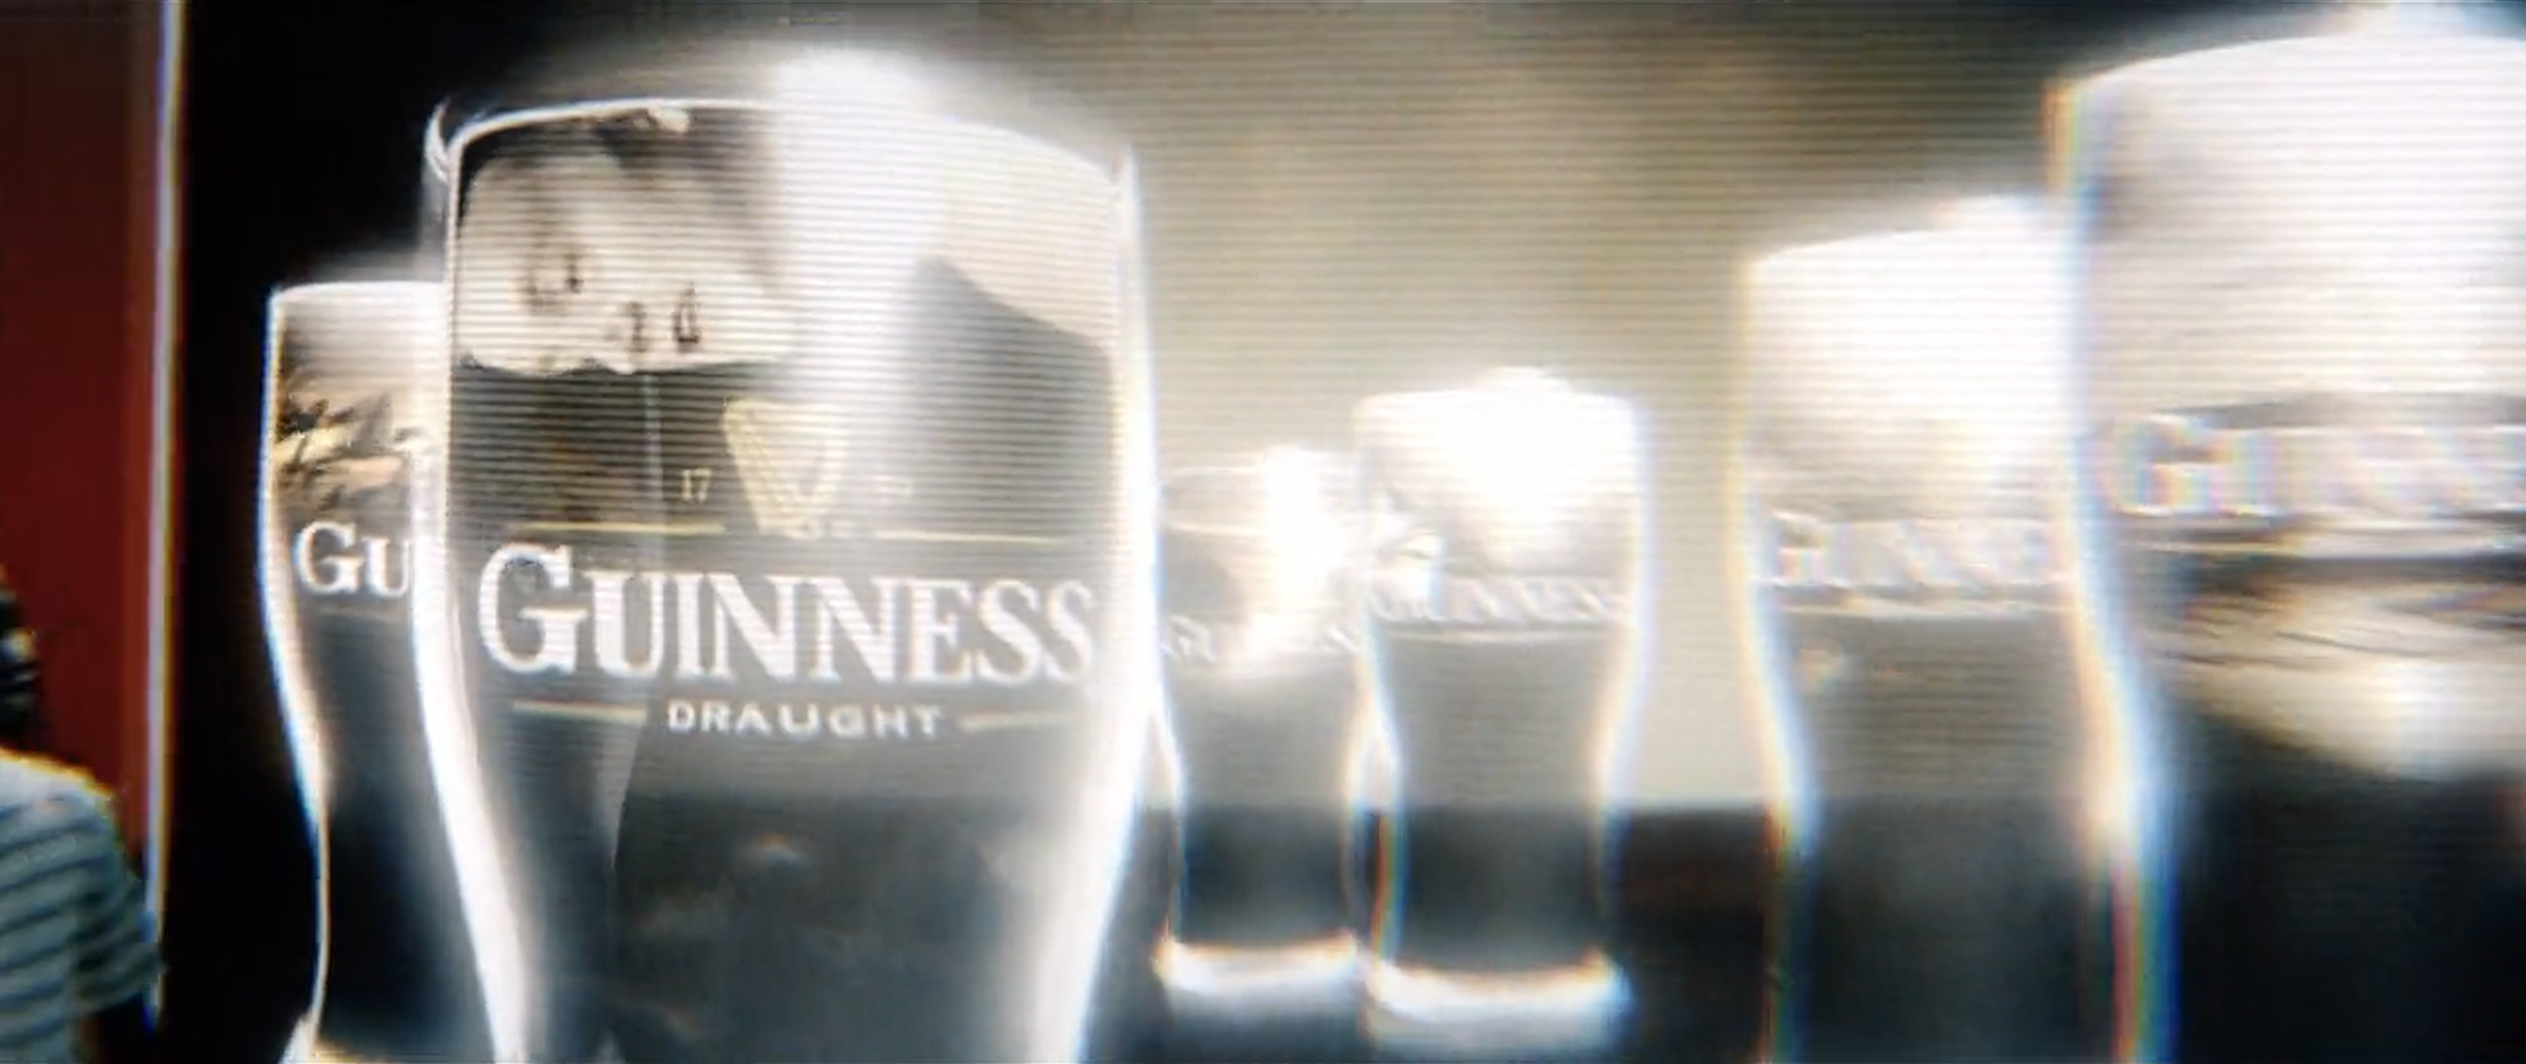
\includegraphics[width=.9\linewidth]{./images/guinness-personalised-advertising-to-john.png}
\caption{A Guinness advertisement that calls out to John by his name, and tells him, "You can use a Guinness right about now."}
\end{figure}

However, the film only shows John Anderton being advertised to in such
a way, and we don't hear the personalised advertisements targetted at
other people, so it is possible that the advertisements can only
be heard by the person that the advertisement
is targetted to.

 \newpage

This does not change how intrusive and invasive the personalised
advertisements are. The fact that all of your purchases are tied to your
identity in the film is a privacy nightmare as there is no doubt
that your purchase history is being sold and shared with other
companies to improve the quality of personalised advertising.
Private companies are also accountable to the law of the country
or state that they are operating in, which means the government
have easy access to all of this information to track and survey you.

\begin{center}
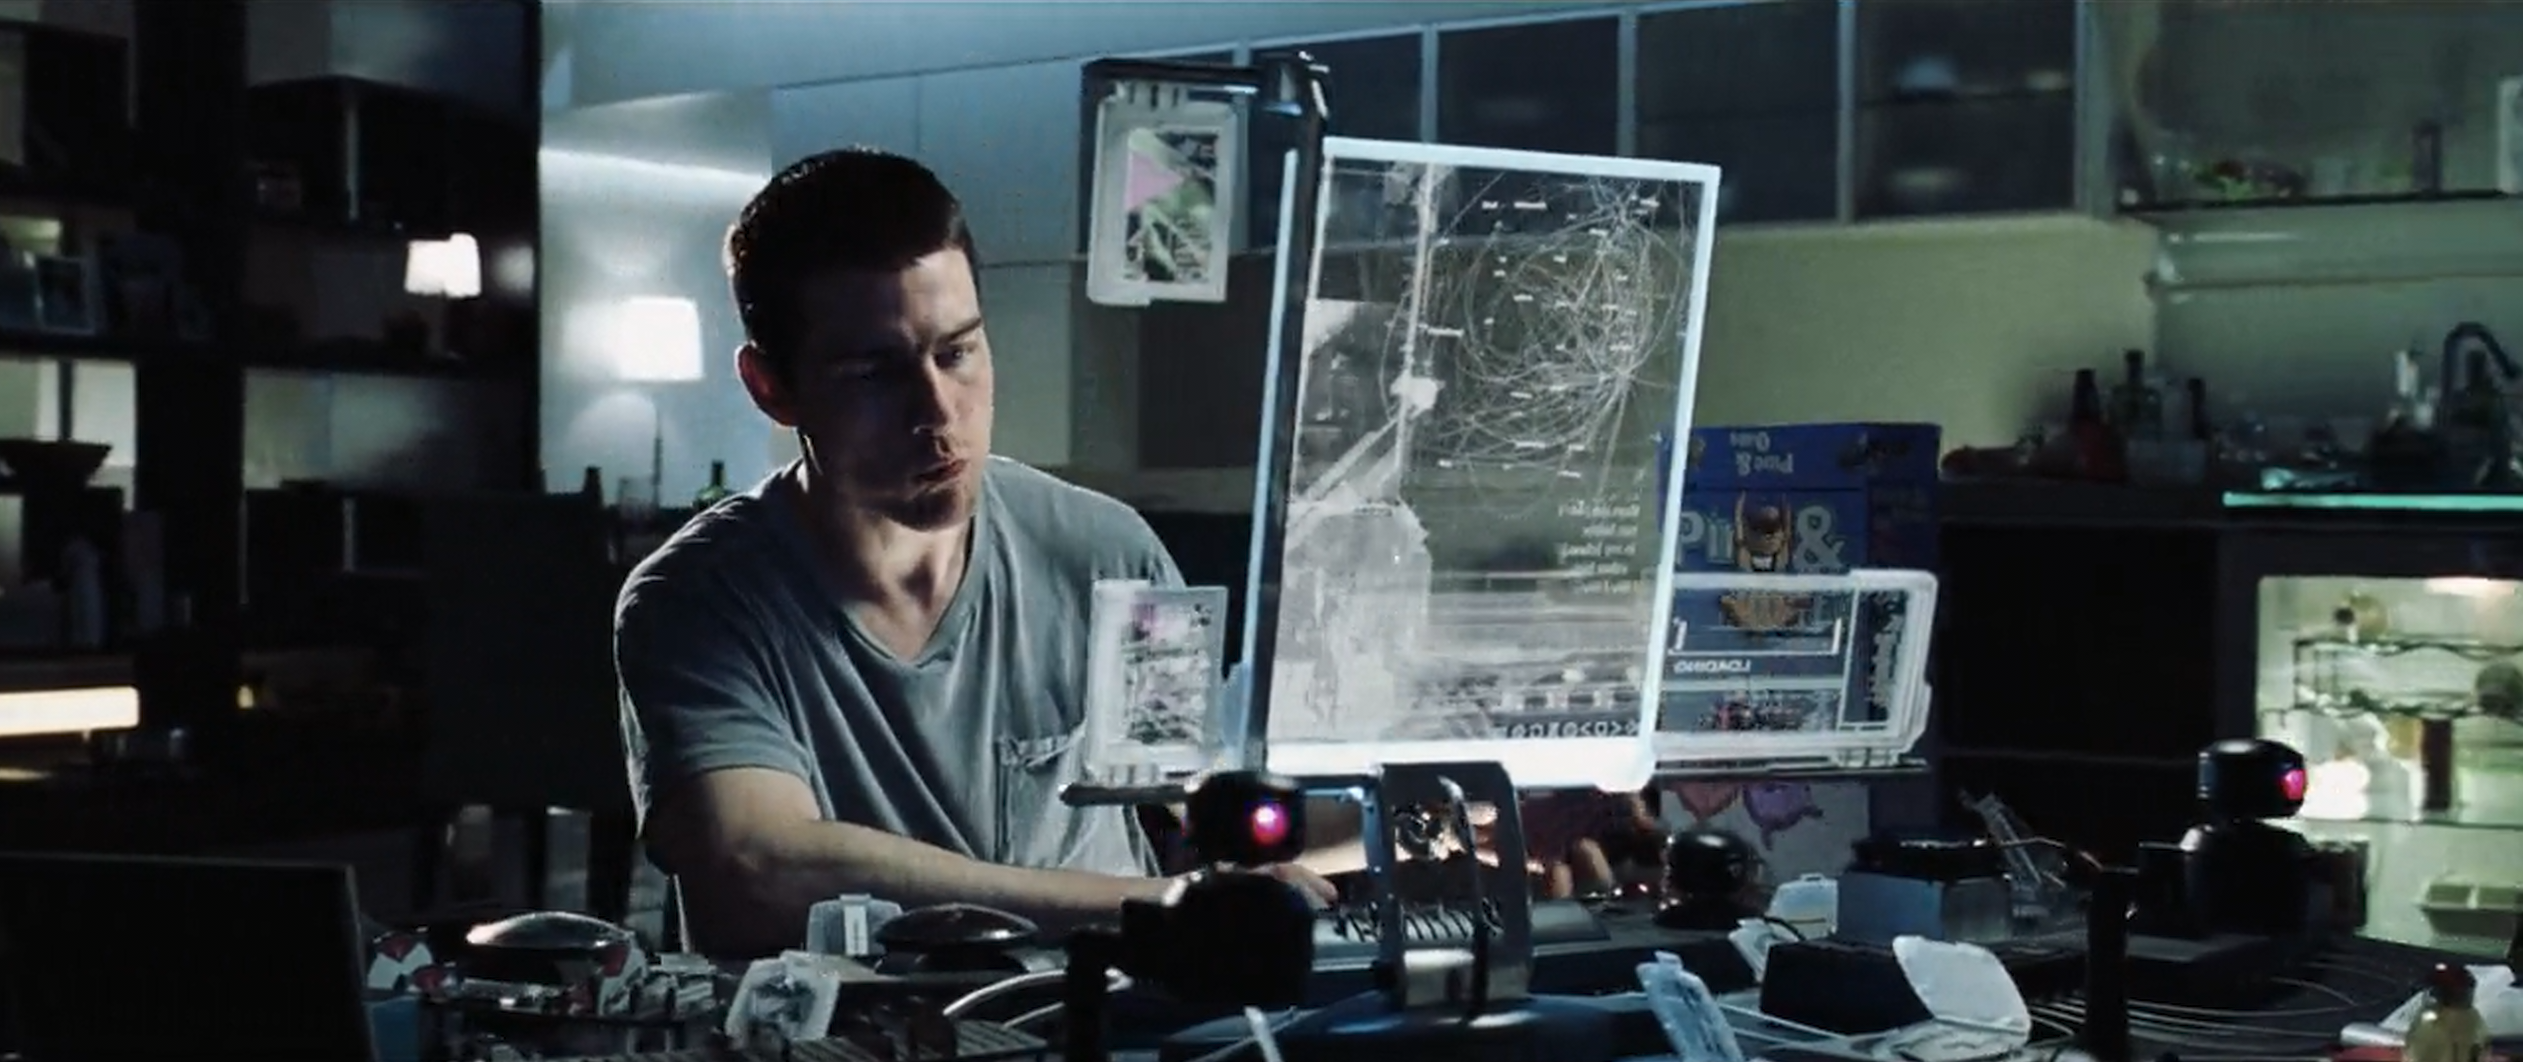
\includegraphics[width=.9\linewidth]{./images/cereal-box-advertising-to-john.png}
\captionof{figure}{The cereal box advertising to John.}
\end{center}

\begin{figure}[htbp]
\centering
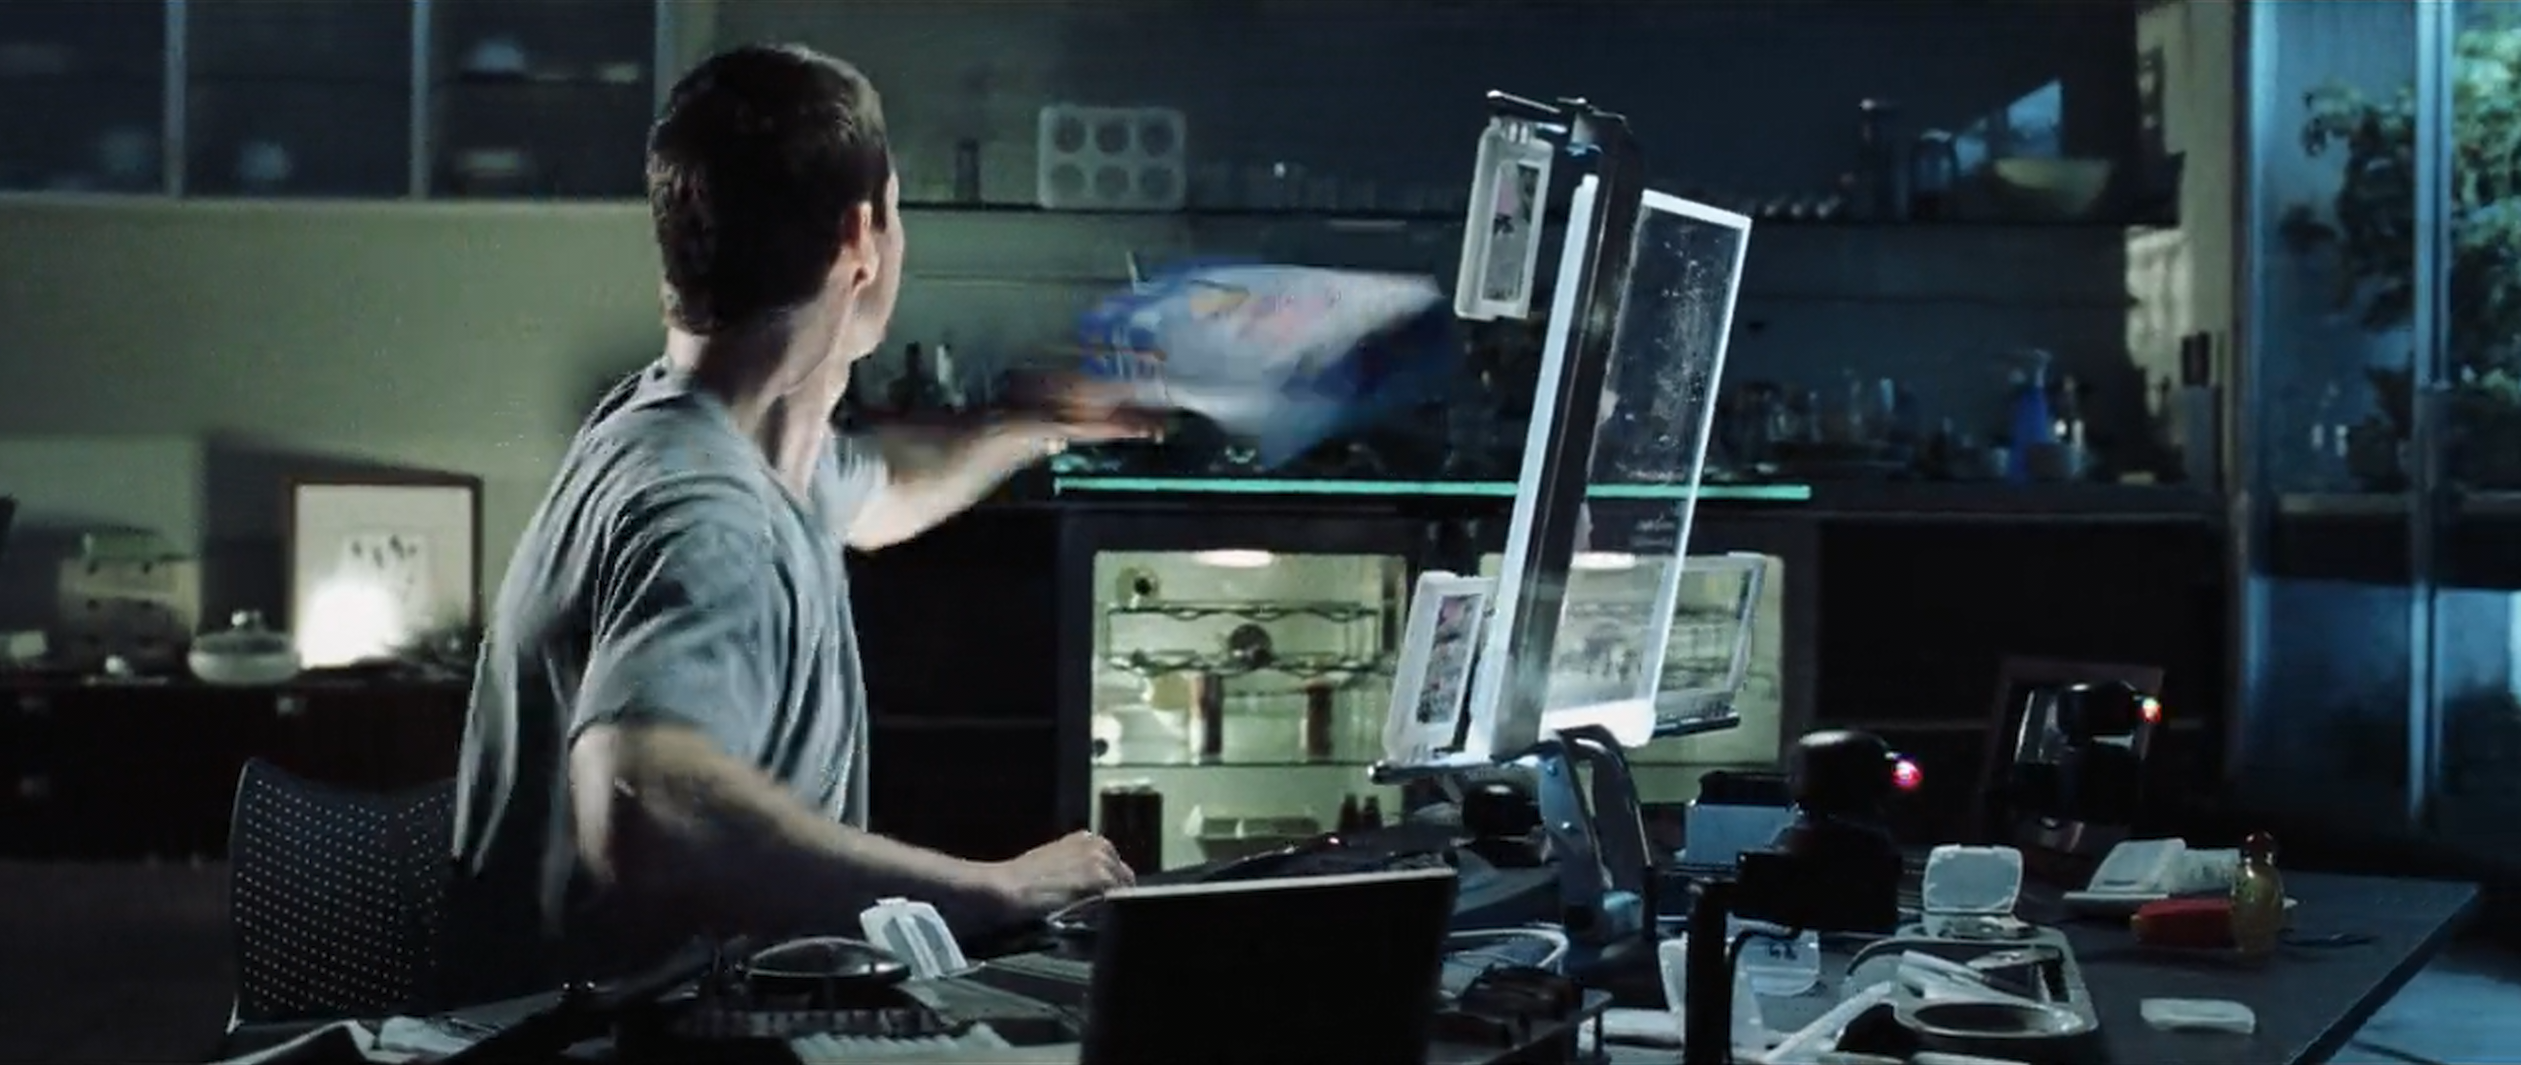
\includegraphics[width=.9\linewidth]{./images/john-throwing-the-cereal-box-away.png}
\caption{John throws the cereal box away after it continues to advertise to him. Honestly, I would do the same after experiencing such intrusive advertising.}
\end{figure}

 \newpage

The scene of the cereal box advertising to John, when he is trying to
have a meal, shows how intrusive this kind of personalised
advertising is. John cannot escape advertising even in
his home, and even after he has already bought the product, shows
that everything has been commodified and there are
no sacred spaces.  \\

We are already seeing personalised advertising in the real
world, we just haven't gone to the extent depicted in the film.
We currently do not have the level of physical tracking present
in the real world with iris or face scanners, but we already have
digital identifiers created and set by trackers.
Most websites nowadays, except for open-source websites, are filled with
trackers that set cookies to identify the user. These scripts are usually
made by big advertising companies like Google, Microsoft and Facebook.
Since most people live quite a large portion of their lives online,
a lot of information is gleaned from tracking the user's
browsing and search history.  \\

Most website owners want to make money from people visiting their site,
so they include these advertising scripts and trackers from these big
advertising companies, which makes it possible for the tracker to keep
a log of your browsing and search history to target advertising to you.
This data is also sufficient to build a profile of
you, which is then sold to data brokers who will sell that data
to other companies, usually advertising companies, to better
target advertising to you. For example, Google might sell your data
to a data broker, and Facebook would buy that data so that they can
tailor the advertising on their platform to
your preferences and tastes.  \\

\begin{figure}[htbp]
\centering

\includegraphics[width=.9\linewidth]{./images/tracking-cookie.png}
\caption{An example of a tracking cookie from Microsoft.}
\end{figure}

 \newpage

This kind of advertising has not only become digitally intrusive,
with auto-playing video advertisements blocking content
and assaulting your ears, it is also a way for
private companies and the government to survey you without your consent
and knowledge. Those cookie banners you see on websites are
not considered informed consent since most people
just accept them without reading anything.
Most websites also automatically allow trackers by default,
and the shady omnipresent "necessary cookies"
could contain tracking cookies, and must be enabled,
so people's data are still being collected and sold without their
consent or knowledge. The worst part is that websites
do not need to ensure that user cookie preferences are being followed,
and can still set cookies as they wish, as the user would not know any
better. Whatever option you choose on the cookie banner may not even
matter at all, as it is up to the website developer to program
their website to respect your cookie preferences. This is illegal
under the EU's ePrivacy directive, better known as the
EU's "cookie law" (\citeprocitem{2}{EU, 2024}), but it is difficult to enforce,
so most sites would get away with doing such things.

\begin{center}
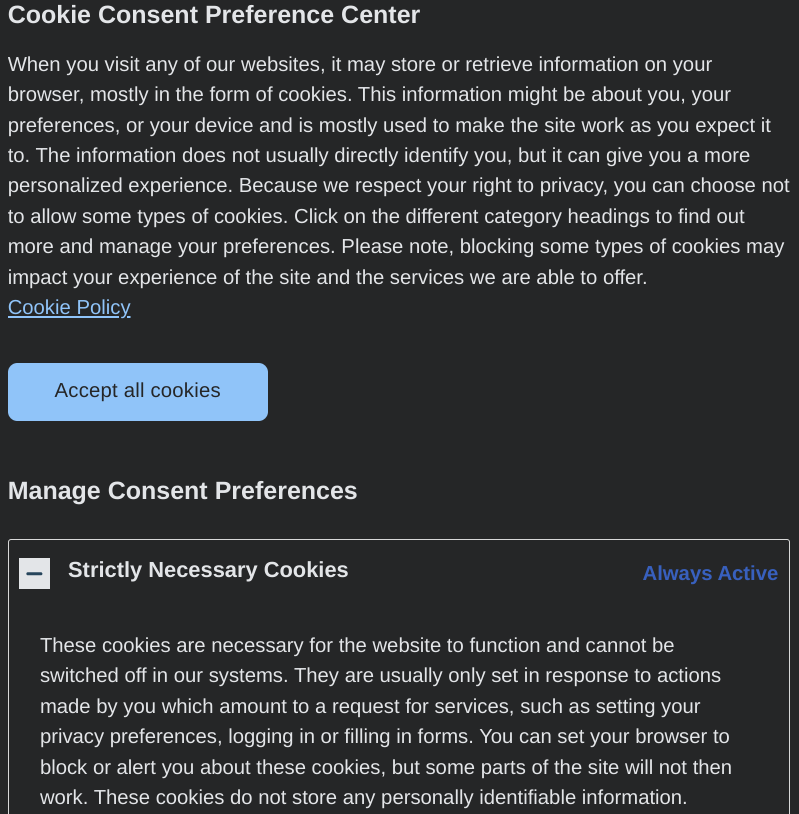
\includegraphics[width=.9\linewidth]{./images/stack-overflow-cookie-banner.png}
\captionof{figure}{An example of a cookie banner, retrieved from \href{https://stackoverflow.com/}{StackOverflow}. You can see that the "Accept all cookies option" is always displayed prominently to entice the user to click it, and the "strictly necessary cookies" is always active.}
\end{center}

 \newpage

\subsection{Government surveillance and tracking}
\label{sec:org9f39775}
In the film, government surveillance is akin to the surveillance
done by an authoritarian regime like the Chinese Communist Party (CCP).
With iris scanners everywhere to track people's every move,
the government knows exactly where every citizen is.
This amount of tracking and surveillance is arguably necessary for
Precrime to be effective, as without it, it would be far more
difficult to stop murders, especially crimes of passion.  \\

\begin{figure}[htbp]
\centering
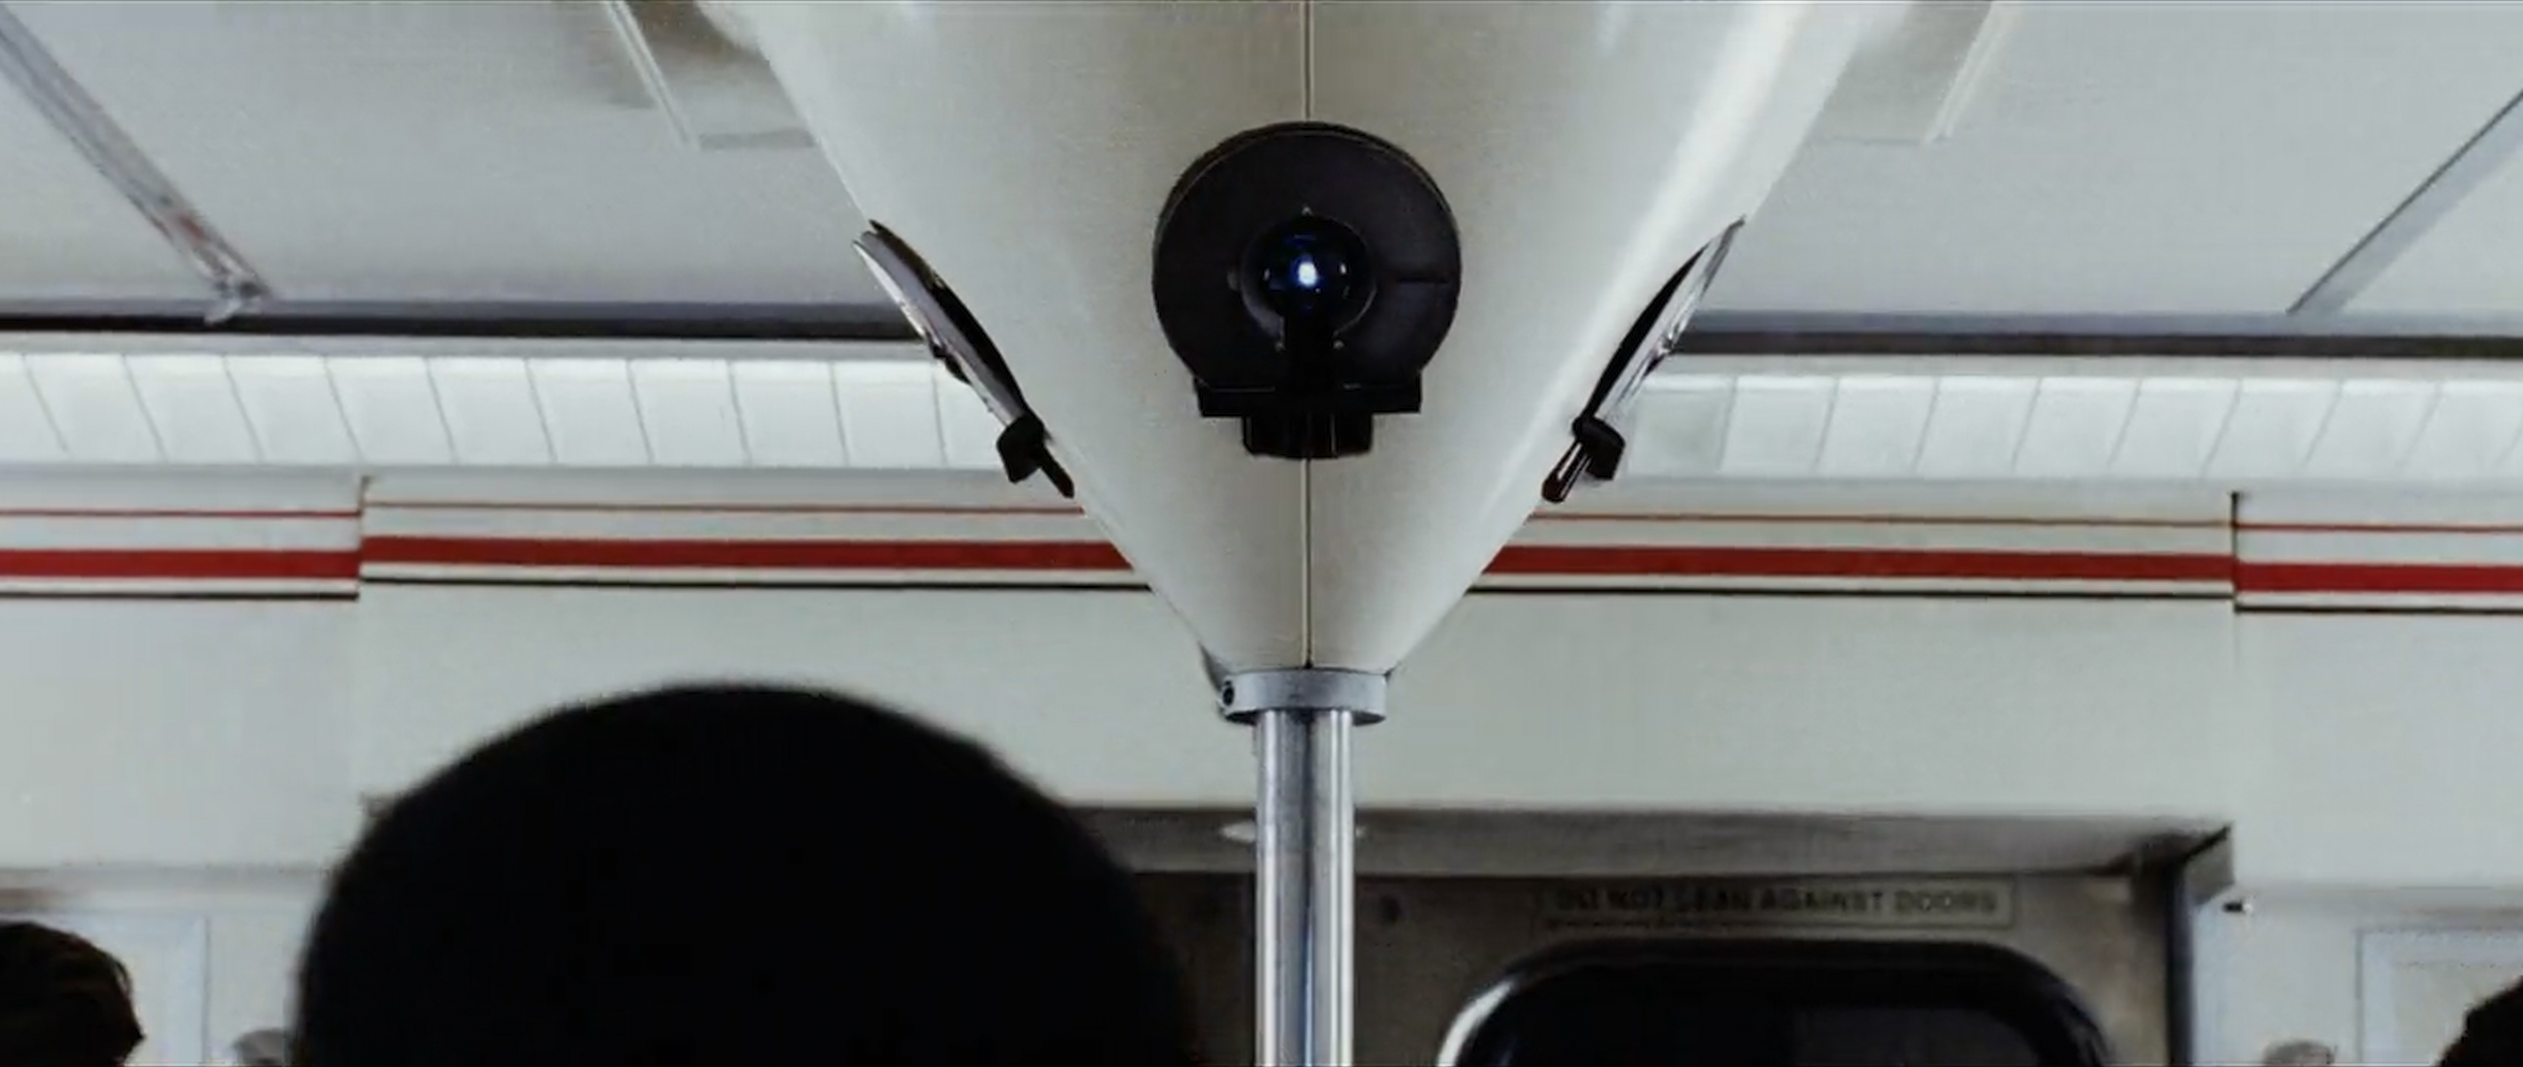
\includegraphics[width=.9\linewidth]{./images/iris-scanner-on-the-train-used-to-track-people.png}
\caption{The iris scanner on the train tracks people who take the train, which gives John's location away to the police department.}
\end{figure}

 \newpage

However, with the government holding such sensitive information about
its citizens, it is prone to abuse, especially if the government changes.
With such information, the government can easily target and persecute
any dissenters to shut them up or make an example of them.
Furthermore, the government may not be the only one with access to
such sensitive information. Employees in the department who
want to do something malicious can very easily do so.
Malicious actors could also hack into government databases to gain access
and use the information for harm.  \\

Unfortunately, the reality is far worse than the depiction in the
film. In the movie, the government is at least considered somewhat
"benevolent" and does not abuse its power to silence dissenters
and political rivals. This has happened far too often in reality,
with the prime example being the CCP. The CCP has placed
surveillance cameras equipped with facial recognition technology everywhere
in China to track their citizens. As of August 2023, China has over 700 million
surveillance cameras (\citeprocitem{4}{Kaur, 2023}),
one camera for every two citizens.
The CCP also places surveillance cameras in the homes of dissidents
(\citeprocitem{8}{Staff, 2013}), likely without their knowledge,
so that the CCP can track them anywhere, and in real-time.
Of course, the CCP doesn't just track and survey these dissidents
for nothing, they arrest these people when they speak up against the CCP.
Wikipedia has a long list of detained and jailed Chinese dissidents
(\citeprocitem{13}{Wikipedia, 2024}).

\subsection{Unwarranted police search}
\label{sec:org801bbb6}
In the film, the police seemingly have the power to enter people's homes
and search their homes and scan their irises whenever they want,
and there is seemingly nothing the people can do about it.
This is not the case in most countries, as the police will need to
either obtain a search warrant or receive your consent before they
can legally enter your home. The fact that the residents do not protest
or resist when the police spider robots enter their homes is mortifying,
as it suggests that they have grown accustomed to the invasion of
privacy by law enforcement. The only resident who protested
the police intrusion into her home was complaining about the
spider robots scaring her children, and said nothing about
the police spider robots being able to access their home willy-nilly.

\begin{center}
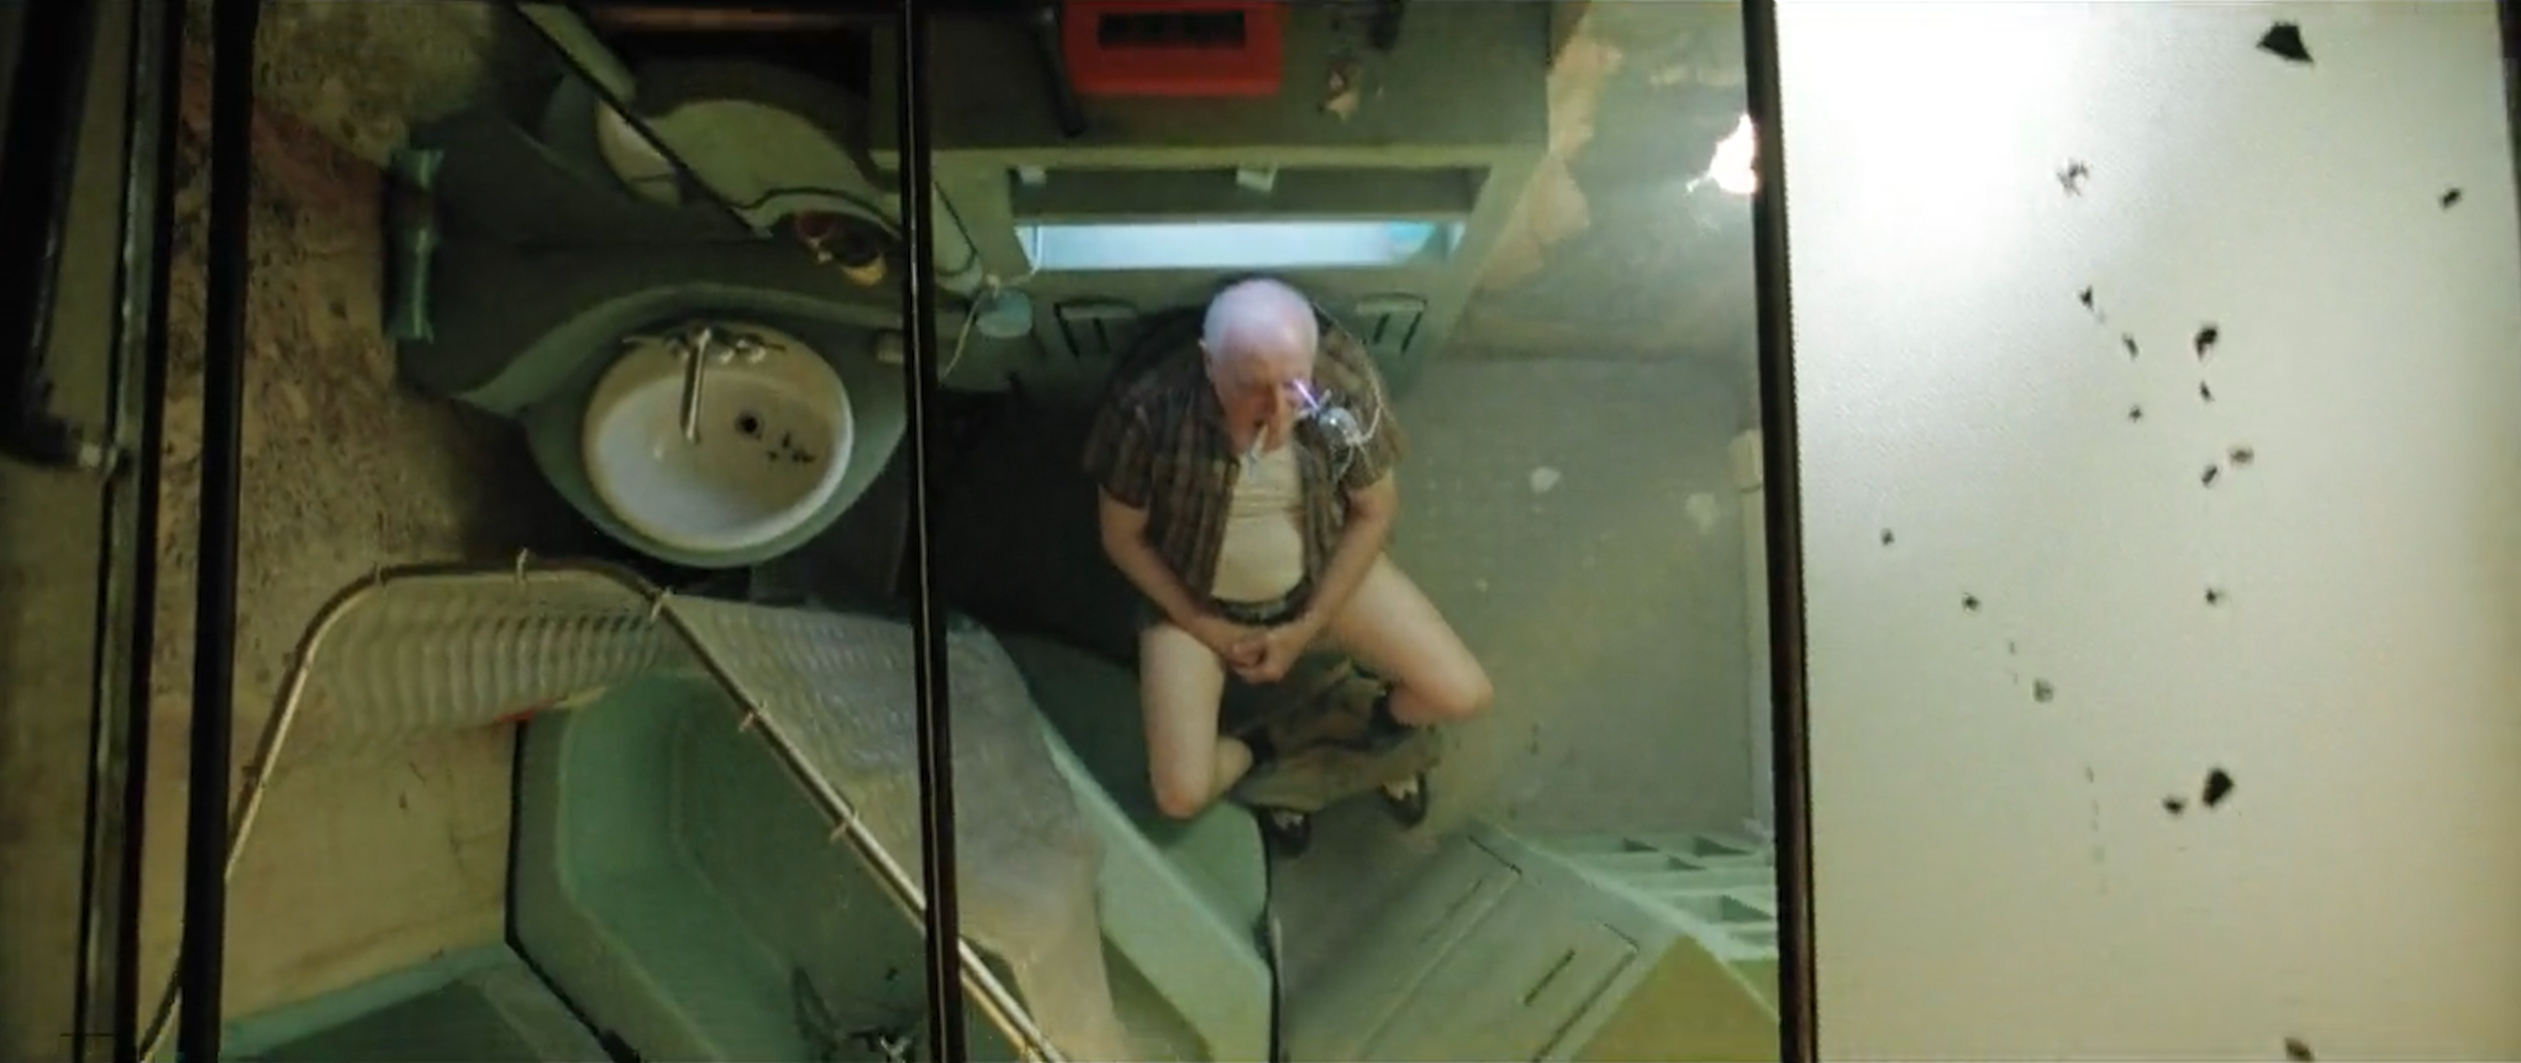
\includegraphics[width=.9\linewidth]{./images/man-getting-his-iris-scanned-while-on-the-toilet.png}
\captionof{figure}{One of the police spider bots scanning an old man's irises when he is sitting on the toilet. This is a massive invasion of privacy.}
\end{center}


\begin{center}
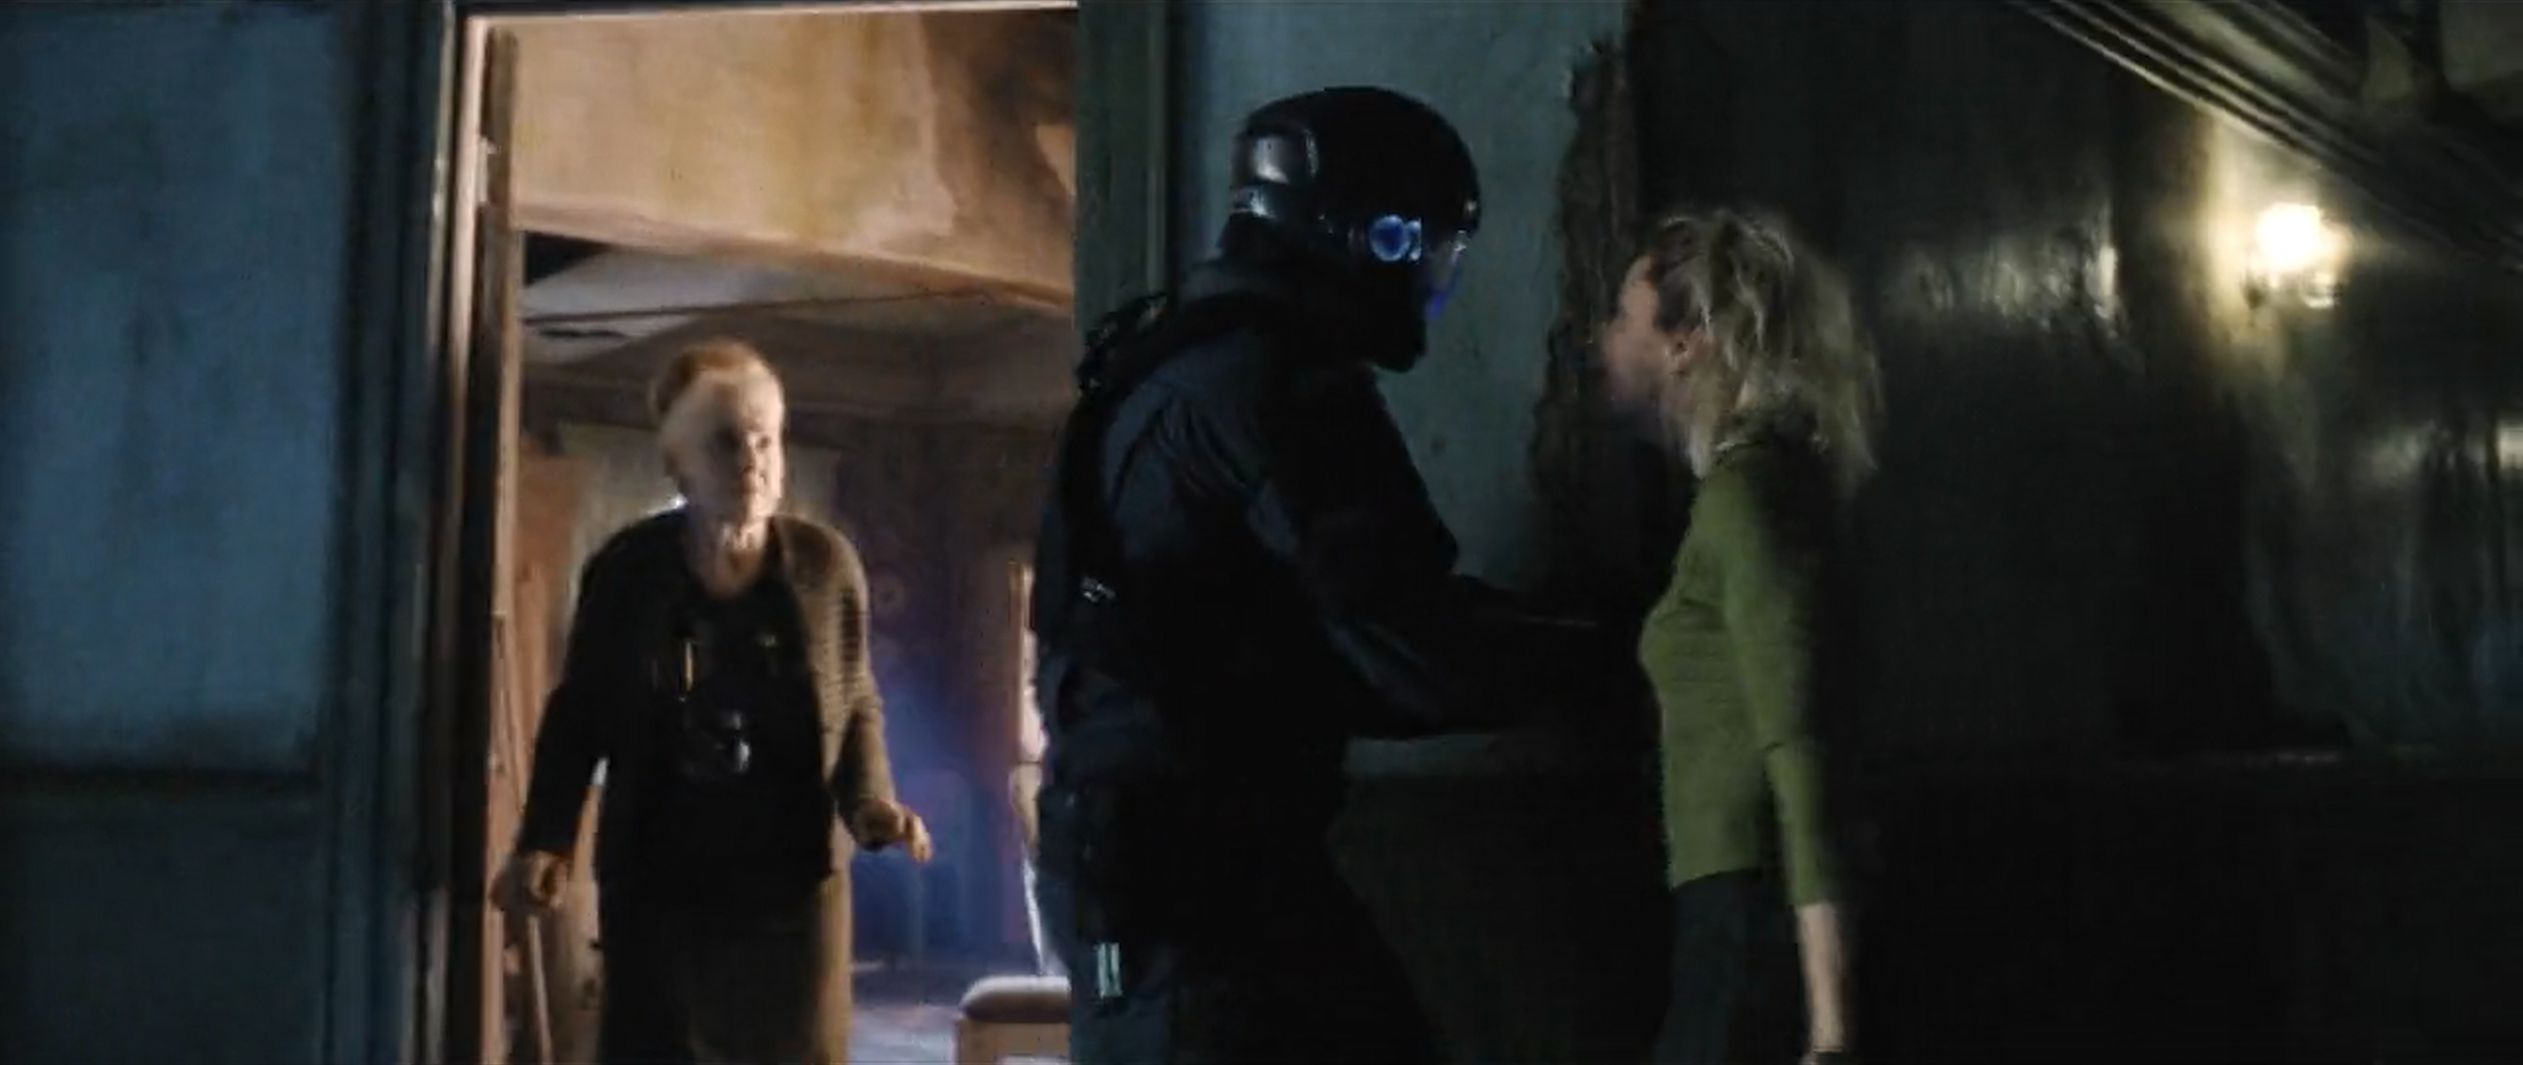
\includegraphics[width=.9\linewidth]{./images/resident-complaining-about-the-spider-robots.png}
\captionof{figure}{The resident complaining about the spider robots terrifying her children.}
\end{center}

\section{Ownership rights}
\label{sec:org3f6e753}
Ownership is defined as the state of legal possession and control over
property. The reasonable understanding of ownership is that you own
whatever item you have purchased, and hence should be able to
do as you please with the item you have purchased, without any
restrictions. This also means that you should have full control over
the item you have purchased and that nobody else should have that
level of control without your permission, since you own the item.
This understanding of ownership will be the definition of the concept
of ownership and ownership rights for this section of the essay.

\subsection{Remote control of consumer products}
\label{sec:org666997e}
In the film, it seems like most cars on the road are driverless,
and are fully autonomous. It also seems like these cars are controlled
by a centralised system which oversees and controls all cars,
as evidenced by the extremely fast and smooth traffic flow
and the incredibly close evasive manoeuvres done by the cars in almost
bumper-to-bumper traffic.  \\

While this allows for a transport system that is highly efficient and
optimised, such centralised control over all vehicles on the road means
that the users of the car have absolutely no control over what their
car does, and cannot do anything they please with the vehicle.
These vehicles may not even be considered private vehicles, since they
operate more like a public transport system, but everyone
has a private space inside a vehicle. People just "purchase" a private
space inside this public transport system, instead
of owning the mode of transport, the car.  \\

However, it seems people in the film indeed "own" the
vehicle they drive, as evidenced by John being able to override the
vehicle locator on his car. Page 62 of the script also states that
John is driving his personal vehicle and not a police issue.

 \newpage

\begin{figure}[htbp]
\centering
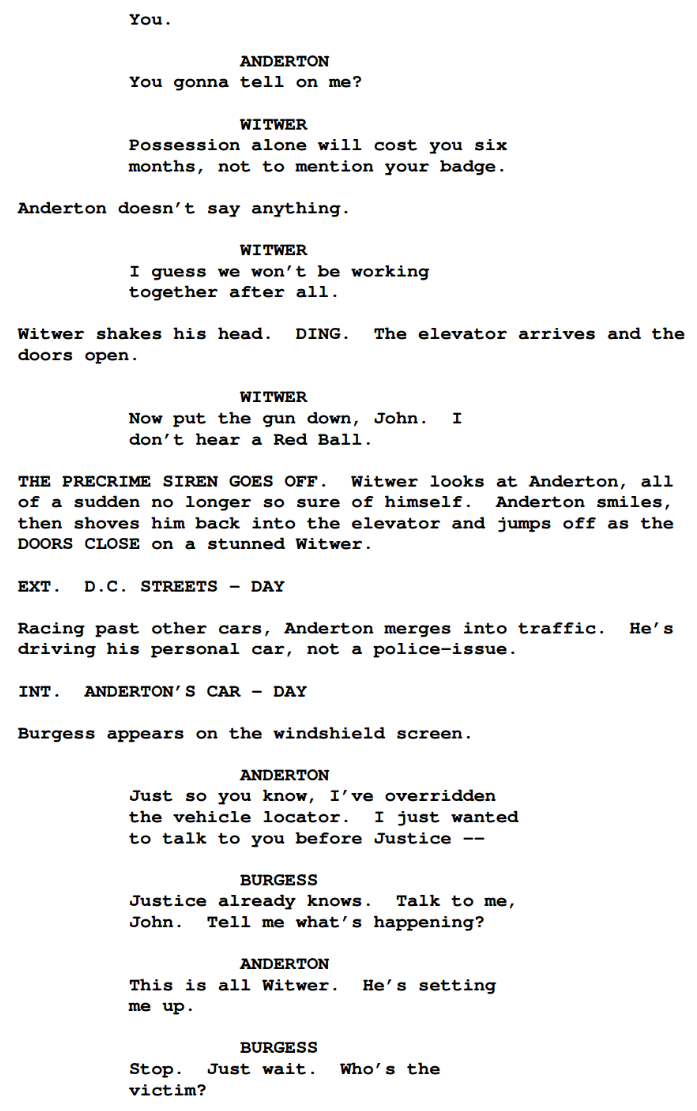
\includegraphics[height=36em]{./images/minority-report-script-page-62.png}
\caption{Page 62 of the script of "Minority Report"}
\end{figure}

Despite John having disabled the vehicle locator, it seems like either
the government or the vehicle manufacturer was able to lock the vehicle
down and forcefully reroute the vehicle to any destination.
This means that John does not have full control over his
vehicle, and cannot do as he pleases with it. Hence, by
the definition of ownership mentioned above, he does not
truly own his vehicle.

\begin{center}
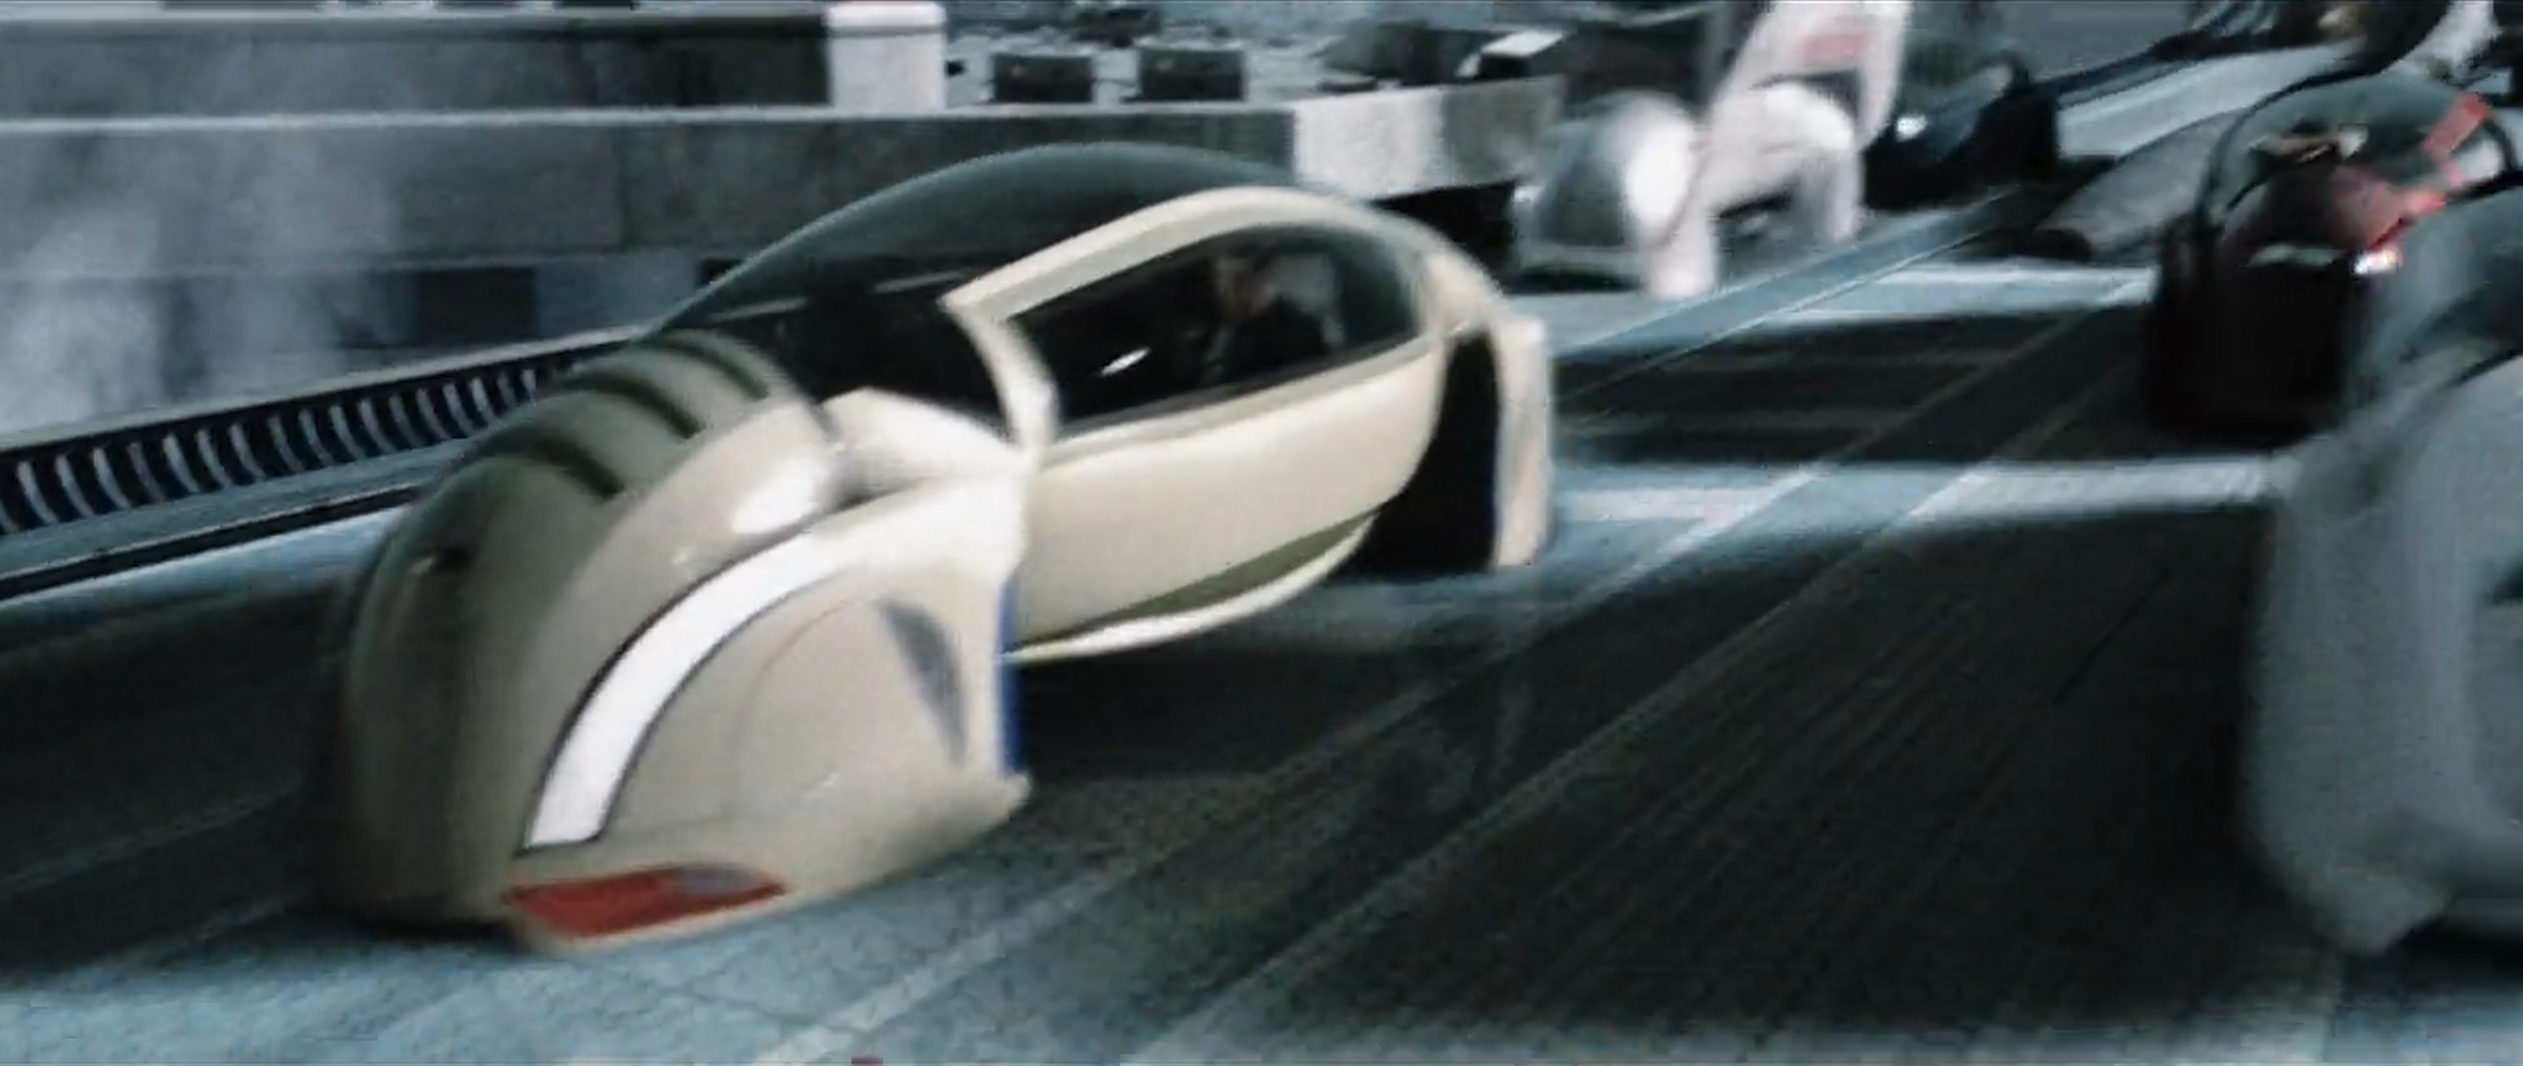
\includegraphics[width=.9\linewidth]{./images/john-locked-out-of-his-car-and-redirected.png}
\captionof{figure}{John Anderton is locked out of his own car and the car is forcefully redirected to his office.}
\end{center}

Unfortunately, this is not just science fiction, as such remote control
over consumer products are already implemented in the real world.
Granted, our current technology does not allow companies or the
government to reroute your vehicle, but some companies have
incredible amounts of control over your vehicle. A prime example of such
a company is Tesla. Tesla can pretty much do anything to
a customer's vehicle remotely. During Hurricane Irma, Tesla remotely
extended the range of some Florida vehicles by unlocking the
full battery capacity of the car so drivers could escape the
hurricane (\citeprocitem{5}{Liptak, 2017}). There are a lot of negative examples as
well, such as Tesla remotely disabling autopilot on a car that was
purchased second-hand (\citeprocitem{9}{Statt, 2020}) and Tesla remotely reducing
the range on a vehicle by 30\% (\citeprocitem{11}{Tangermann, 2022}).  \\

This does not just apply to physical goods like cars and is especially
common with digital goods, like movies and games.
An example is Sony removing purchased movies from
customers' libraries due to licensing issues, twice
(\citeprocitem{6}{Niemeyer, 2023}; \citeprocitem{7}{Porter, 2022}).
Most video games purchased through a gaming platform like Steam
and Epic Games also carries the same risk, with the only exception being
\href{https://www.gog.com/}{GOG.com} as they provide you directly with the
installer for the game without Digital Rights Management (DRM) software.

 \newpage

With an increasing number of companies looking towards subscription
to earn a consistent stream of revenue from their customers,
our ability to own items as consumers is gradually being eroded.
Companies have far more control over the products we purchase
now than ever before, and a lot of them are abusing it to earn more
revenue, while making their services worse for customers.
Roku TV recently updated its terms of service, forcing users
to go through arbitration for any disputes with the company.
Users who did not accept this change were locked out of using
their TVs, that they purchased, through a software update (\citeprocitem{3}{Harding, 2024}).
Ring, a security camera company owned by Amazon, was
recently fined \$5.8 million for failing to protect their users' data.
Employees and third-party contractors could view,
download and transfer users' video data (\citeprocitem{1}{Bartz, 2023}).
Tesla employees also admitted that they had access to the video
feed of customers' cars and were sharing those videos
(\citeprocitem{10}{Stecklow et al., 2023}).

 \newpage

\section{Slavery and child labour}
\label{sec:org087ddfc}

\begin{figure}[htbp]
\centering
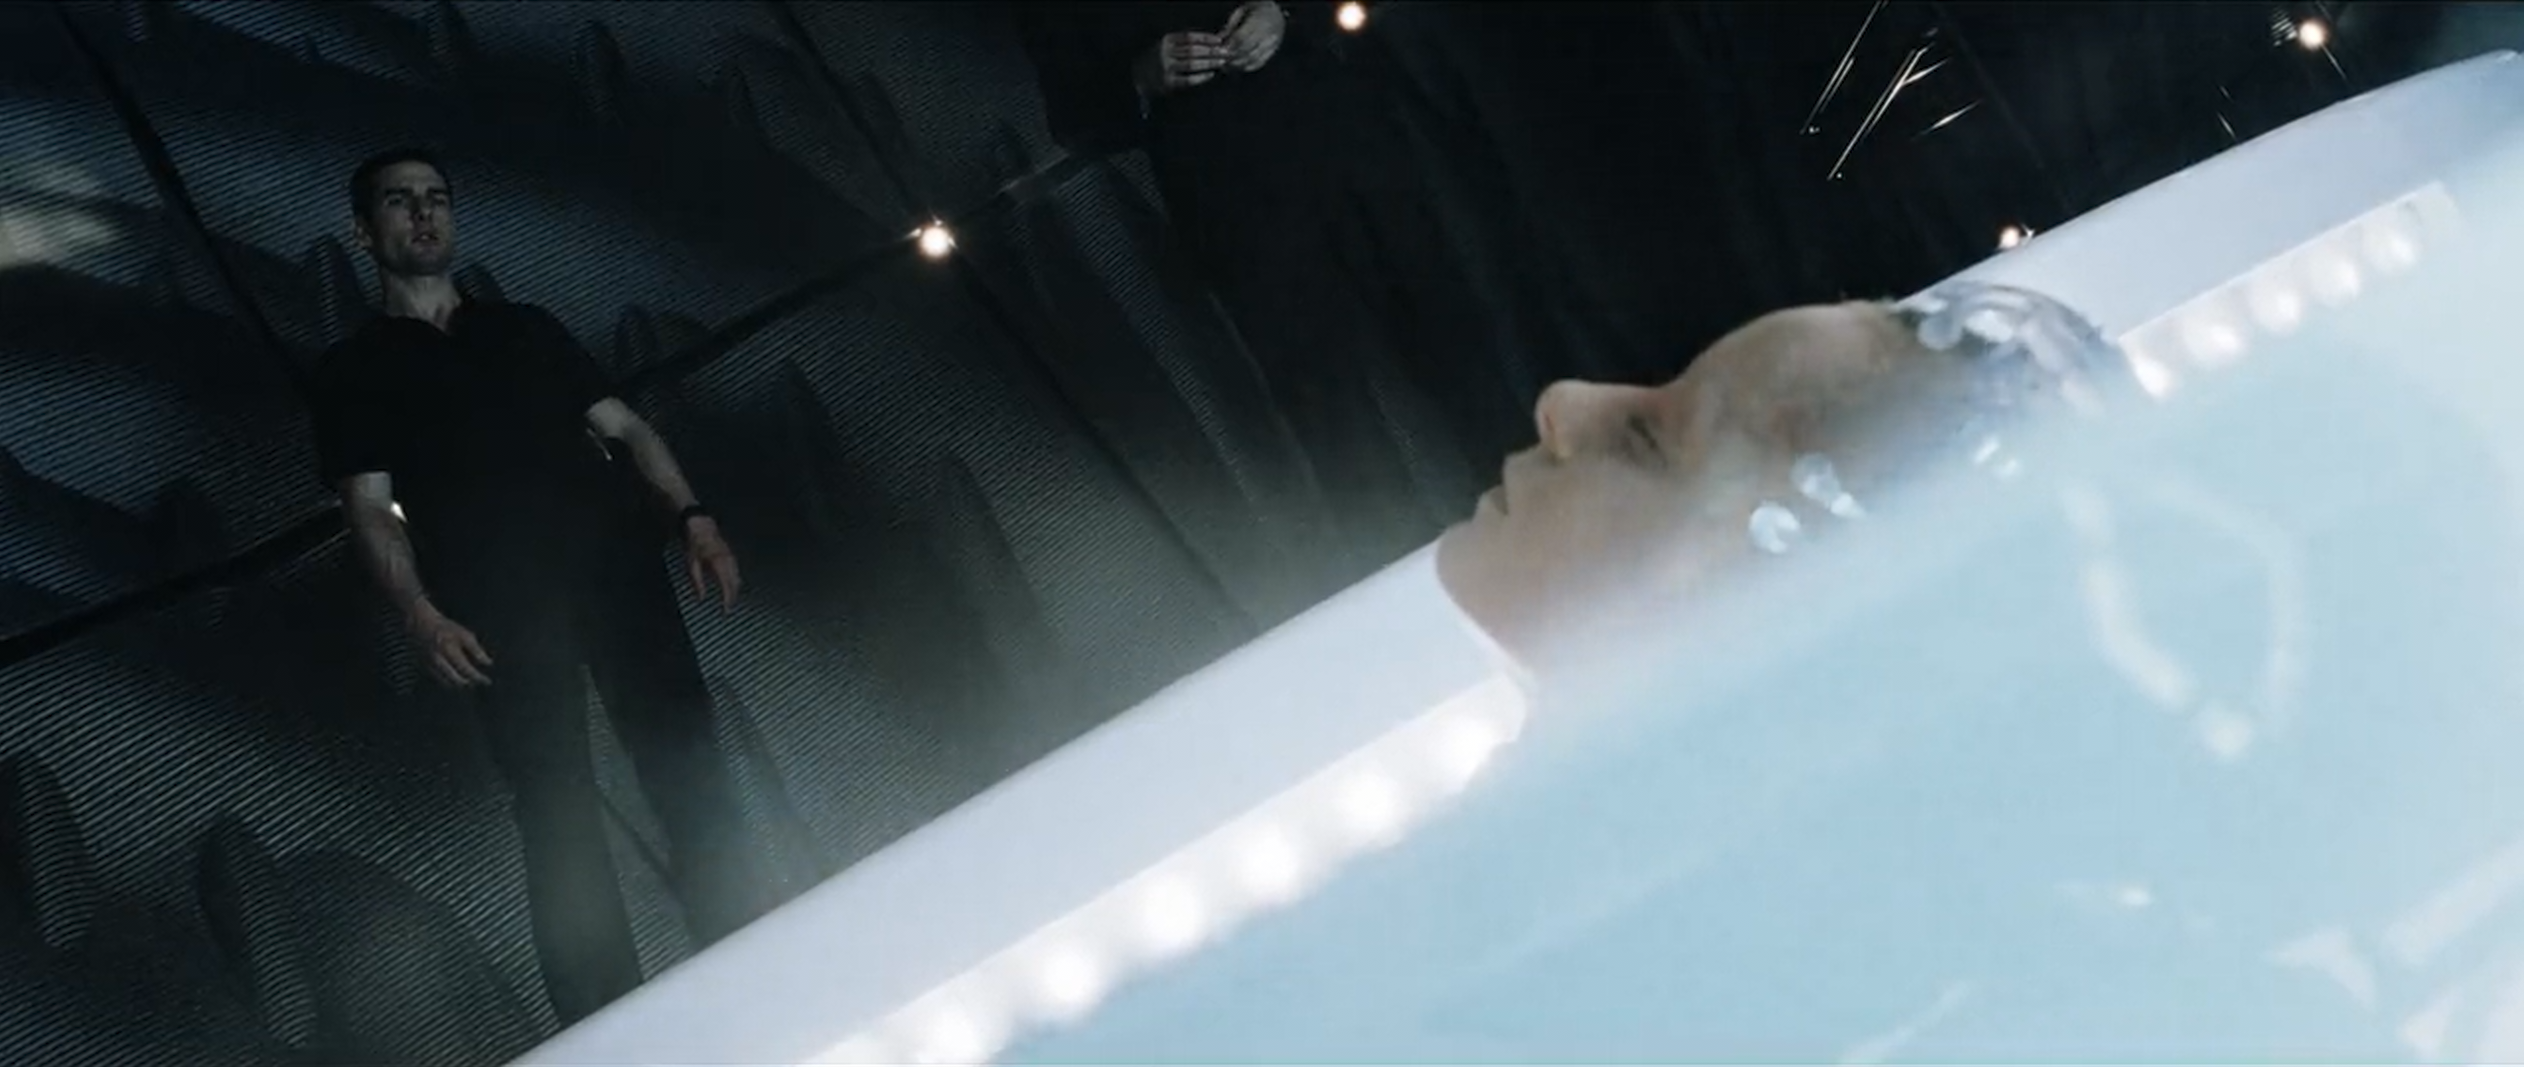
\includegraphics[width=.9\linewidth]{./images/precog-scene-where-john-says-to-not-think-of-them-as-human.png}
\caption{The scene where John says, "It helps if you don't think of them (the Precogs) as human."}
\end{figure}

At the beginning of the film, John states that it is better to not
think of the Precogs as humans, which made me believe that the Precogs
were some form of android that was developed to have precognition.
John also seemed to think the Precogs were engineered as well,
as he seeks Dr. Hineman wanting to fake a prevision, calling the
Precogs her "invention".
However, it is revealed by Dr. Hineman that the Precogs were
children who suffered from brain damage because of their
parents' use of the drug Neuroin, and developed precognition as a
side effect of the damage.

\begin{figure}[htbp]
\centering
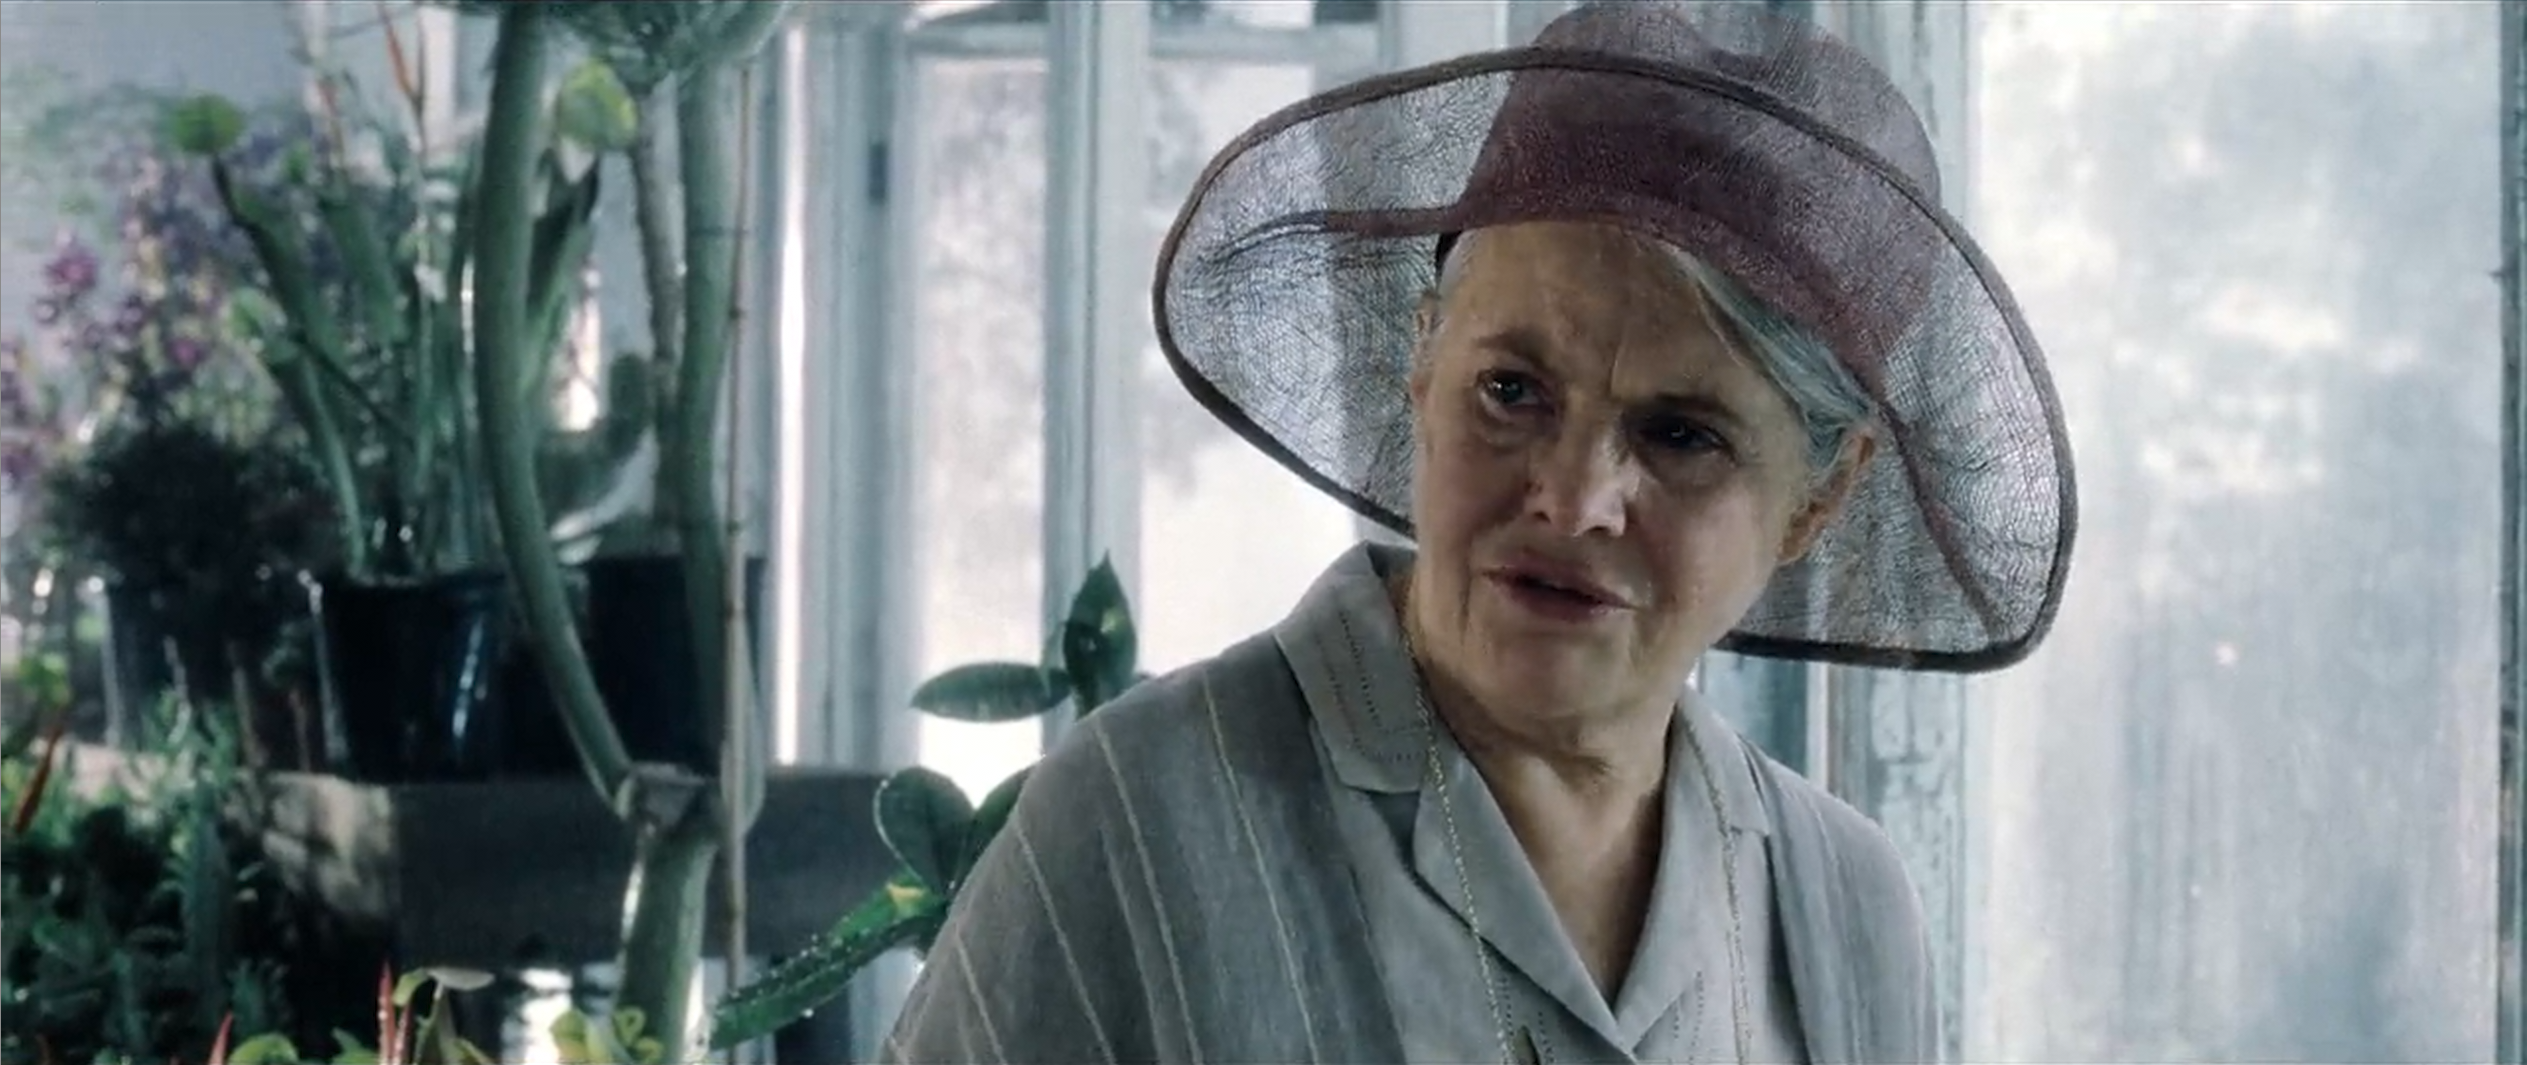
\includegraphics[width=.9\linewidth]{./images/dr-hineman-telling-john-the-truth-about-the-precogs.png}
\caption{Dr. Hineman telling John the truth about the Precogs.}
\end{figure}

 \newpage

This meant that the Precogs were essentially enslaved children that
are forced to work for the Precrime police department, which means
the government was actively participating in slavery and using
child labour, which are crimes in the real world.
This is made even more evident by the fact that Lamar Burgess kills
Anne Lively, the mother of Agatha Lively, the strongest of the three
Precogs, so he can keep Agatha for use in the
Precrime program.  \\

This is slavery and child labour, and in a pretty terrible
form as well, as the Precogs are forced to
watch the previsions of violent murders
continuously, while they are stuck in a tank, unable to move,
and hooked up to machines. All the while being pumped full of drugs
and nutrients to keep them alive. Agatha may even be subjected to
sexual abuse by the caretaker Wally.

\begin{figure}[htbp]
\centering
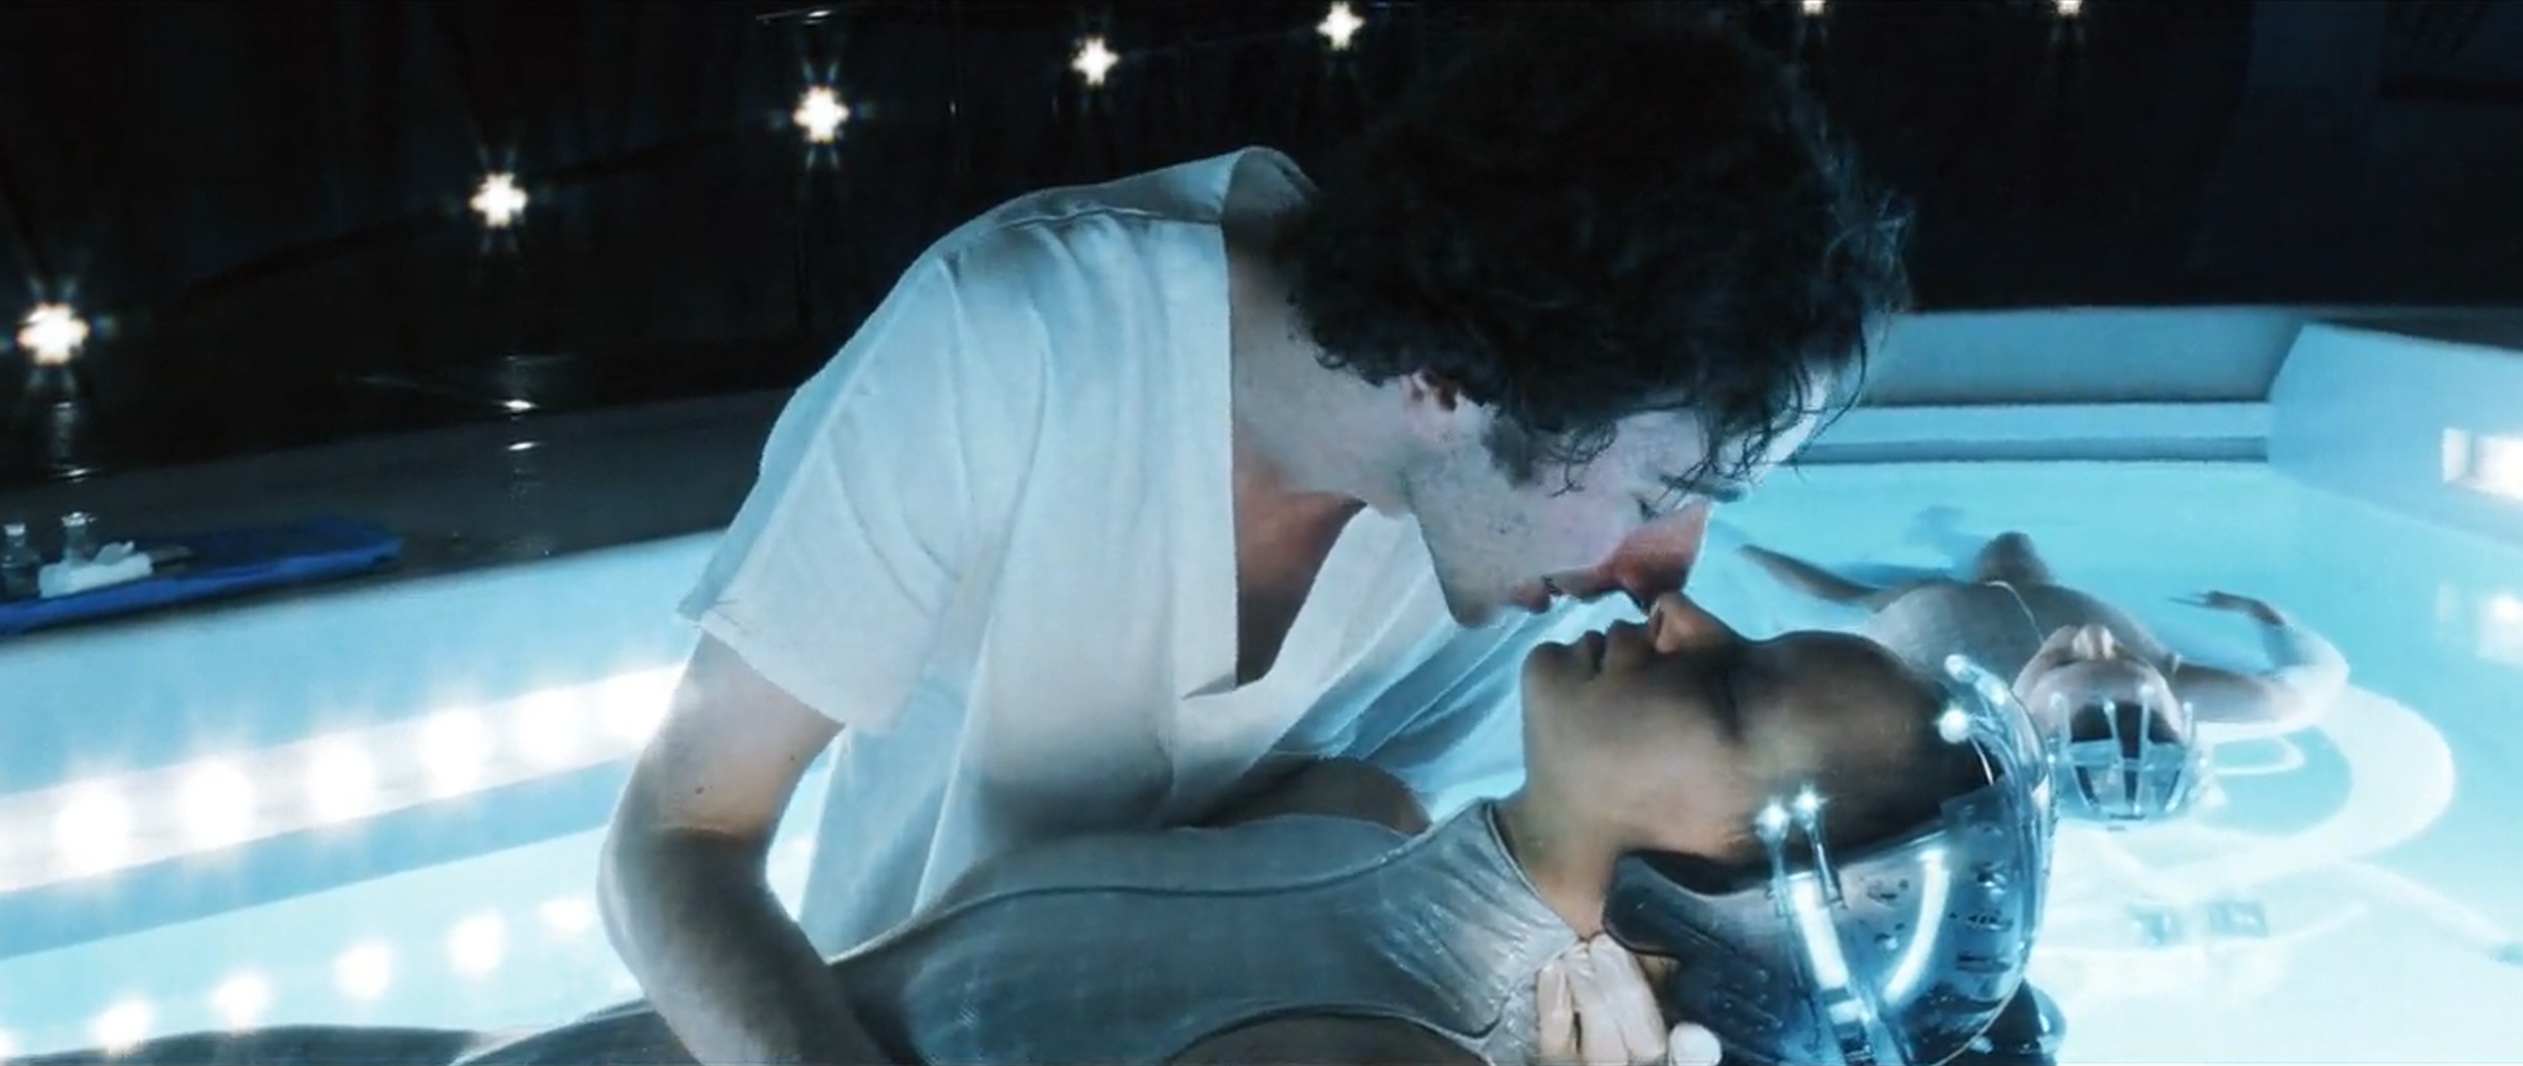
\includegraphics[width=.9\linewidth]{./images/wally-creepy-behaviour-after-getting-agatha-back.png}
\caption{The scene of Wally after getting Agatha back. His behaviour is pretty creepy, especially kissing her, considering that Agatha is still a child.}
\end{figure}

 \newpage

\section{Conclusion}
\label{sec:org903c212}
In summary, there are a lot of issues with the world depicted
in "Minority Report", and the Precrime system isn't as justifiable
as it seems at first. The many issues with surveillance and
government control make me, as a person who values privacy
and freedom, view it as a dystopia. The enslavement of children
and forcing them to work for the greater good is also morally
questionable.  \\

Sadly, some issues brought up in the film are already
happening in the real world, like government surveillance
and control in countries like China, the erosion of ownership
by companies, and not enough is being done to fight against it.
Very few people truly value their privacy and freedom,
and are happy with companies collecting and selling their data
to the highest bidder, which I can understand, as privacy
usually comes at the cost of inconvenience in a world where
every single thing (digitally at least) is trying to track you.
I fear it may be too late when people are finally fed up and
start pushing back, only to find that nothing will change because
these tech and advertising companies have complete control
over everything and will persecute anyone who doesn't follow
the status quo. Hopefully, we will never reach that point, but
only time will tell.

 \newpage

\section{Bibliography}
\label{sec:orgcb5556b}
Below is the list of references used in this essay.  \\

\begin{hangparas}{1.5em}{1}
\hypertarget{citeproc_bib_item_1}{Bartz, D. (2023). Amazon’s ring used to spy on customers, ftc says in privacy settlement | reuters. In \textit{Reuters}. \url{https://www.reuters.com/legal/us-ftc-sues-amazoncoms-ring-2023-05-31/}}

\hypertarget{citeproc_bib_item_2}{EU. (2024). Cookies, the gdpr, and the eprivacy directive. In \textit{Gdpr.eu}. \url{https://gdpr.eu/cookies/}}

\hypertarget{citeproc_bib_item_3}{Harding, S. (2024). “Disgraceful”: Messy tos update allegedly locks roku devices until users give in. In \textit{Ars technica}. \url{https://arstechnica.com/gadgets/2024/03/disgraceful-messy-tos-update-allegedly-locks-roku-devices-until-users-give-in/}}

\hypertarget{citeproc_bib_item_4}{Kaur, D. (2023). After years of dominating facial recognition tech, china is ready to govern it. In \textit{Tech wire asia}. \url{https://techwireasia.com/2023/08/facial-recognition-tech-in-china-will-soon-be-governed/}}

\hypertarget{citeproc_bib_item_5}{Liptak, A. (2017). Tesla extended the range of some florida vehicles for drivers to escape hurricane irma. In \textit{The verge}. The Verge. \url{https://www.theverge.com/2017/9/10/16283330/tesla-hurricane-irma-update-florida-extend-range-model-s-x-60-60d}}

\hypertarget{citeproc_bib_item_6}{Niemeyer, K. (2023). Playstation is removing hundreds of discovery shows that users already purchased. In \textit{Business insider}. Business Insider. \url{https://www.businessinsider.com/playstation-removes-hundreds-of-purchased-discovery-shows-from-library-2023-12}}

\hypertarget{citeproc_bib_item_7}{Porter, J. (2022). Playstation store removes purchased movies from libraries after service shutdown. In \textit{The verge}. The Verge. \url{https://www.theverge.com/2022/7/8/23199861/playstation-store-film-tv-show-removed-austria-germany-studiocanal}}

\hypertarget{citeproc_bib_item_8}{Staff, T. W. (2013). The week at a glance.international. In \textit{Theweek}. The Week. \url{https://theweek.com/articles/468149/week-glanceinternational}}

\hypertarget{citeproc_bib_item_9}{Statt, N. (2020). Tesla remotely disables autopilot on used model s after it was sold. In \textit{The verge}. The Verge. \url{https://www.theverge.com/2020/2/6/21127243/tesla-model-s-autopilot-disabled-remotely-used-car-update}}

\hypertarget{citeproc_bib_item_10}{Stecklow, S., Cunningham, W., \& Jin, H. (2023). Tesla workers shared sensitive images recorded by customer cars | reuters. In \textit{Reuters}. \url{https://www.reuters.com/technology/tesla-workers-shared-sensitive-images-recorded-by-customer-cars-2023-04-06/}}

\hypertarget{citeproc_bib_item_11}{Tangermann, V. (2022). Tesla cuts car’s range by 30\%, demands \$4,500 to get it back. In \textit{Futurism}. Futurism. \url{https://futurism.com/tesla-range-reduce-remote}}

\hypertarget{citeproc_bib_item_12}{Warren, S. D., \& Brandeis, L. D. (1890). In \textit{Right to privacy}. \url{https://faculty.uml.edu/sgallagher/Brandeisprivacy.htm}}

\hypertarget{citeproc_bib_item_13}{Wikipedia. (2024). List of chinese dissidents. In \textit{Wikipedia}. Wikimedia Foundation. \url{https://en.wikipedia.org/wiki/List_of_Chinese_dissidents}}\bigskip
\end{hangparas}
\end{document}
